\pdfoutput = 1

\documentclass[10pt]{article}
% % set pdf figure transparency problems
% \pdfpageattr {/Group << /S /Transparency /I true /CS /DeviceRGB>>}

\usepackage[usenames,dvipsnames,svgnames,table]{xcolor}
\usepackage{amsmath, amsthm, amssymb, bbm, bm}
\usepackage{enumerate}
\usepackage{graphicx}
\usepackage{float}      % figure inside minipage,
\usepackage{wrapfig, subcaption}
\usepackage[margin=0cm]{caption}
\usepackage[titletoc, toc]{appendix}
\usepackage{microtype}
\usepackage{blindtext}
\usepackage{tabularx}
\usepackage{booktabs,colortbl}

\usepackage[boxruled, vlined, linesnumbered]{algorithm2e}
\SetAlFnt{\small}
\SetAlCapFnt{\small}
\SetAlCapNameFnt{\small}
\usepackage{algorithmic}
\algsetup{linenosize=\tiny}

\let\oldnl\nl% Store \nl in \oldnl
\newcommand{\nonl}{\renewcommand{\nl}{\let\nl\oldnl}}% Remove line number for one line

\usepackage[bookmarks=false]{hyperref}
%\usepackage[hyperpageref]{backref}
\hypersetup{
colorlinks=true, linkcolor=Sepia, citecolor=Sepia, filecolor=magenta, urlcolor=black,
}
\usepackage{url, bookmark}

\renewcommand{\qed}{\hfill \mbox{\raggedright \rule{0.1in}{0.1in}}}

% math macros
\newcommand{\reals}{\mathbb{R}}
\newcommand{\naturals}{\mathbb{N}}
\newcommand{\complex}{\mathbb{C}}

\newcommand{\abs}[1]{\ensuremath \left| #1 \right|}
\newcommand{\norm}[1]{\ensuremath \lVert#1\rVert}
\newcommand{\given}{\, \vert \,}
\providecommand{\cal}[1]{\ensuremath \mathcal{#1}}
\newcommand{\ag}[1]{\ensuremath \left\langle#1\right\rangle}
\providecommand{\OO}{\mathcal{O}}
\newcommand{\indep}{\protect\mathpalette{\protect\independenT}{\perp}}
\def\independenT#1#2{\mathrel{\rlap{$#1#2$}\mkern2mu{#1#2}}}
\newcommand{\trace}{\trm{tr}}
\newcommand{\kron}{\otimes}
\DeclareMathOperator*{\argmin}{argmin}
\DeclareMathOperator*{\argmax}{argmax}

% shortcuts
\newcommand{\aeq}[1]{\begin{align} #1 \end{align}}
\newcommand{\aeqs}[1]{\begin{align*} #1 \end{align*}}
\newcommand{\beq}[1]{\begin{equation}#1\end{equation}}
\newcommand{\beqs}[1]{\begin{equation*}#1\end{equation*}}

\newcommand{\trm}[1]{\mathrm{#1}}
\newcommand{\enum}[2][(a)]{\begin{enumerate}[#1]{#2}\end{enumerate}}
\newcommand{\clist}[1]{\begin{itemize}\setlength{\itemsep}{0pt}
\setlength{\parsep}{0pt}
{#1}\end{itemize}}
\newcommand{\ilist}[1]{\begin{itemize}{#1}\end{itemize}}
\newcommand{\bmat}[1]{\begin{bmatrix}#1\end{bmatrix}}
\newcommand{\mpage}[2]{\begin{center}
\begin{minipage}{#1}#2\end{minipage}\end{center}}
\newcommand{\la}{\ \leftarrow\ }
\newcommand{\ra}{\rightarrow}
\providecommand\f[2]{\ensuremath \frac{#1}{#2}}
\providecommand\rbrac[1]{\ensuremath \left(#1\right)}
\providecommand\sqbrac[1]{\ensuremath \left[#1\right]}
\providecommand\cbrac[1]{\ensuremath \left\{#1\right\}}

\newcommand{\deriv}[1]{\f{d}{d #1}\ }
\newcommand{\pderiv}[1]{\f{\partial}{\partial #1}\ }

\newtheorem{theorem}{Theorem}
\newtheorem{proposition}[theorem]{Proposition}
\newtheorem{lemma}[theorem]{Lemma}
\newtheorem{corollary}[theorem]{Corollary}
\newtheorem{problem}[theorem]{Problem}

\theoremstyle{definition}
\newtheorem{definition}[theorem]{Definition}
\newtheorem{example}[theorem]{Example}
\newtheorem{note}[theorem]{Note}
\newtheorem{remark}[theorem]{Remark}
\newtheorem{assumption}[theorem]{Assumption}

\renewcommand{\P}{\trm{P}}
\newcommand{\E}{\mathbb{E}}
\newcommand{\corr}{\textrm{cross-corr}\ }
\providecommand{\ones}{\mathbbm{1}}
\providecommand{\ind}{{\bf 1}}
\providecommand{\nnot}[1]{\overline{#1}}
\providecommand{\oor}{\vee}
\providecommand{\aand}{\wedge}
\renewcommand{\implies}{\Rightarrow}
\newcommand{\convp}{\overset{P}{\to}}
\newcommand{\convd}{\overset{\DD}{\to}}

\newcommand{\s}{\sigma}
\newcommand{\w}{\omega}
\renewcommand{\r}{\rho}
\renewcommand{\t}{\tau}
\renewcommand{\th}{\theta}
\renewcommand{\a}{\alpha}
\newcommand{\p}{\phi}
\newcommand{\e}{\epsilon}
\renewcommand{\b}{\beta}
\newcommand{\g}{\gamma}
\renewcommand{\d}{\delta}
\newcommand{\D}{\Delta}
\newcommand{\z}{\zeta}
\renewcommand{\L}{\Lambda}
\renewcommand{\l}{\lambda}
\newcommand{\G}{\Gamma}
\renewcommand{\S}{\Sigma}
\newcommand{\Th}{\Theta}

\def \XX {\mathcal{X}}
\def \LL {\mathcal{L}}
\def \DD {\mathcal{D}}
\def \FF {\mathcal{F}}
\def \OO {\mathcal{O}}
\def \tOO {\widetilde{\mathcal{O}}}
\def \BB {\mathcal{B}}
\def \PP {\mathcal{P}}

\newcommand{\bR}{\mathbb{R}}
\newcommand{\bN}{\mathbb{N}}
\newcommand{\bZ}{\mathbb{Z}}

\def \rmF {\trm{F}}

\newcommand{\var}{\trm{var}}
\newcommand{\stddev}{\trm{stddev}}
\newcommand{\covar}{\trm{covar}}

\newcommand{\Poissondist}{\trm{Poisson}}
\newcommand{\Berdist}{\trm{Ber}}
\newcommand{\Geomdist}{\trm{Geom}}
\newcommand{\Betadist}{\trm{Beta}}
\newcommand{\Bindist}{\trm{Bin}}
\newcommand{\Gammadist}{\trm{Gamma}}
\newcommand{\InvGammadist}{\trm{InvGamma}}
\newcommand{\Expdist}{\trm{Exp}}

\newcommand{\mozo}{\{-1, 0, 1\}}
\newcommand{\moo}{\{-1, 1\}}
\newcommand{\mooc}{[-1, 1]}
\newcommand{\zoo}{\{0, 1\}}

\newcommand{\data}{\trm{input}}
\newcommand{\convolution}{\trm{conv}}
\newcommand{\maxpool}{\textrm{max-pool}}
\newcommand{\meanpool}{\trm{meanpool}}
\newcommand{\relu}{\trm{relu}}
\newcommand{\dropout}{\trm{dropout}}
\newcommand{\linear}{\trm{linear}}
\newcommand{\softmax}{\trm{softmax}}
\newcommand{\batchnorm}{\trm{batchnorm}}
\newcommand{\block}{\trm{block}}
\usepackage{iclr2017_conference}
\usepackage{mathptmx}

\linespread{1.02}

%\pagestyle{empty}

% save space
\setlength{\floatsep}{0.0in}
\setlength{\textfloatsep}{0.0in}
\setlength{\intextsep}{0.05in}
\setlength{\belowcaptionskip}{0.05in}
\setlength{\abovecaptionskip}{0.05in}
\setlength{\abovedisplayskip}{0.05in}
\setlength{\belowdisplayskip}{0.05in}

% notation goes here
\newcommand\red[1]{{\color{red}#1}}
\newcommand{\entropysgd}{\mathrm{Entropy}\textrm{-}\mathrm{SGD}}
\newcommand{\minibatch}[1]{\Xi^{#1}}
\newcommand{\mnistfc}{\textrm{mnistfc}}
\newcommand{\smallmnistfc}{\textrm{small-mnistfc}}
\newcommand{\charlstm}{\textrm{char-lstm}}
\newcommand{\lenet}{\textrm{LeNet}}
\newcommand{\allcnn}{\textrm{All-CNN-BN}}

\title{Entropy-SGD: Biasing Gradient Descent Into Wide Valleys}

\author{Pratik Chaudhari$^{1}$, Anna Choromanska$^{2}$, Stefano Soatto$^{1}$, Yann LeCun$^{2,3}$, Carlo Baldassi$^{4}$,\\[0.03in]
\textbf{Christian Borgs$^{5}$, Jennifer Chayes$^{5}$, 
Riccardo Zecchina$^{4}$}\\[0.05in]
$^{1}$ Computer Science, University of California, Los Angeles.\\
$^{2}$ Courant Institute of Mathematical Sciences, New York University.\\
$^{3}$ Facebook AI Research, New York.\\
$^{4}$ Politecnico di Torino.\\
$^{5}$ Microsoft Research New England, Cambridge.\\ [0.05in]
{\footnotesize
Email:\ \href{mailto:pratikac@ucla.edu}{pratikac@ucla.edu},
\href{mailto:achoroma@cims.nyu.edu}{achoroma@cims.nyu.edu},
\href{mailto:soatto@cs.ucla.edu}{soatto@cs.ucla.edu},
\href{mailto:yann@cs.nyu.edu}{yann@cs.nyu.edu},
\href{mailto:carlobaldassi@gmail.com}{carlobaldassi@gmail.com}}\\[0.03in]
{\footnotesize
\hspace{0.33in} \href{mailto:borgs@microsoft.com}{borgs@microsoft.com},
\href{mailto:jchayes@microsoft.com}{jchayes@microsoft.com},
\href{mailto:riccardo.zecchina@polito.it}{riccardo.zecchina@polito.it}
}}

% macros to color text and insert margin comments
\setlength{\marginparwidth}{1in}
\newcommand{\pc}[2]{{\color{ForestGreen}#1}\marginpar{\tiny\noindent{\raggedright{\color{Sienna}[PC]}\color{Sienna}{#2} \par}}}
\renewcommand{\ss}[2]{{\color{cyan}#1}\marginpar{\tiny\noindent{\raggedright{\color{BurntOrange}[SS]}\color{BurntOrange}{#2} \par}}}
\newcommand{\ac}[2]{{\color{magenta}#1}\marginpar{\tiny\noindent{\raggedright{\color{magenta}[AC]}\color{magenta}{#2} \par}}}
\newcommand{\todo}[1]{{\color{gray}#1}\marginpar{\tiny\noindent{\raggedright{\color{blue}[TODO]}}}}
\newcommand{\ignore}[1]{}

% uncomment these for submission!
% \renewcommand{\pc}[2]{#1}
% \renewcommand{\ss}[2]{#1}
% \renewcommand{\ac}[2]{#1}
% \renewcommand{\todo}[1]{#1}

\graphicspath{{./fig/}}

%\iclrfinalcopy % Uncomment for camera-ready version
\begin{document}

\maketitle

\begin{abstract}
This paper proposes a new optimization algorithm called $\entropysgd$ for training deep neural networks that is motivated by the local geometry of the energy landscape. Local extrema with low generalization error have a large proportion of almost-zero eigenvalues in the Hessian with very few positive or negative eigenvalues. We leverage upon this observation to construct a local entropy based objective function that favors well-generalizable solutions lying in large flat regions of the energy landscape, while avoiding poorly-generalizable solutions located in the sharp valleys. Conceptually, our algorithm resembles two nested loops of SGD, where we use Langevin dynamics to compute the gradient of the local entropy at each update of the weights. We prove that the local entropy objective function is smoother than the original landscape and use uniform stability to show improved generalization bounds over SGD. Our experiments on competitive baselines demonstrate that $\entropysgd$ leads to generalization performances that compare with state of the art techniques and also has the potential to accelerate training.
\end{abstract}

\section{Introduction}
\label{s:intro}
This paper presents a new optimization tool for deep learning designed to exploit the local geometric properties of the objective function. Consider the histogram in Fig.~\ref{fig:lenet_hessian} showing the spectrum of the Hessian at an extremum discovered by Adam~\citep{kingma2014adam} for a convolutional neural network on MNIST~\citep{lecun1998gradient} with about $47,000$ weights (cf.\@ Sec.~\ref{ss:expt:universality}). It is evident that:
\begin{enumerate}[(i)]
\item a large number of directions ($\approx 94\%$) have near-zero eigenvalues (magnitude less than $10^{-4}$),
\item positive eigenvalues (right inset) have a long tail with the largest one being almost $40$,
\item negative eigenvalues (left inset), which are directions of descent that the optimizer missed, have a much faster decay (the largest negative eigenvalue is only $-0.4$).
\end{enumerate}
Interestingly, this trend is not unique to this particular network. Rather, its qualitative properties are shared across a variety of network architectures, sizes, datasets or optimization algorithms (refer to Sec.~\ref{s:expt} for more experiments). Local minima that generalize well and are discovered by gradient descent lie in ``wide valleys'' of the energy landscape, rather than in sharp isolated minima. \todo{For an intuitive understanding of this phenomenon, imagine a Bayesian prior concentrated at the minimizer of the expected loss, the marginal likelihood of wide valleys under this prior is much higher than narrow, sharp valleys even if the latter are close to the global minimum in training loss.} Almost-flat regions of the energy landscape are robust to data perturbations, noise in the activations, as well as perturbations of the parameters --- all of which are widely-used techniques to achieve good generalization. This suggests that wide valleys should result in better generalization and, indeed, standard optimization algorithms in deep learning --- without being explicitly tailored to do so --- seem to discover exactly that.

\begin{figure}[tbh]
% \vspace*{-0.1in}
\centering
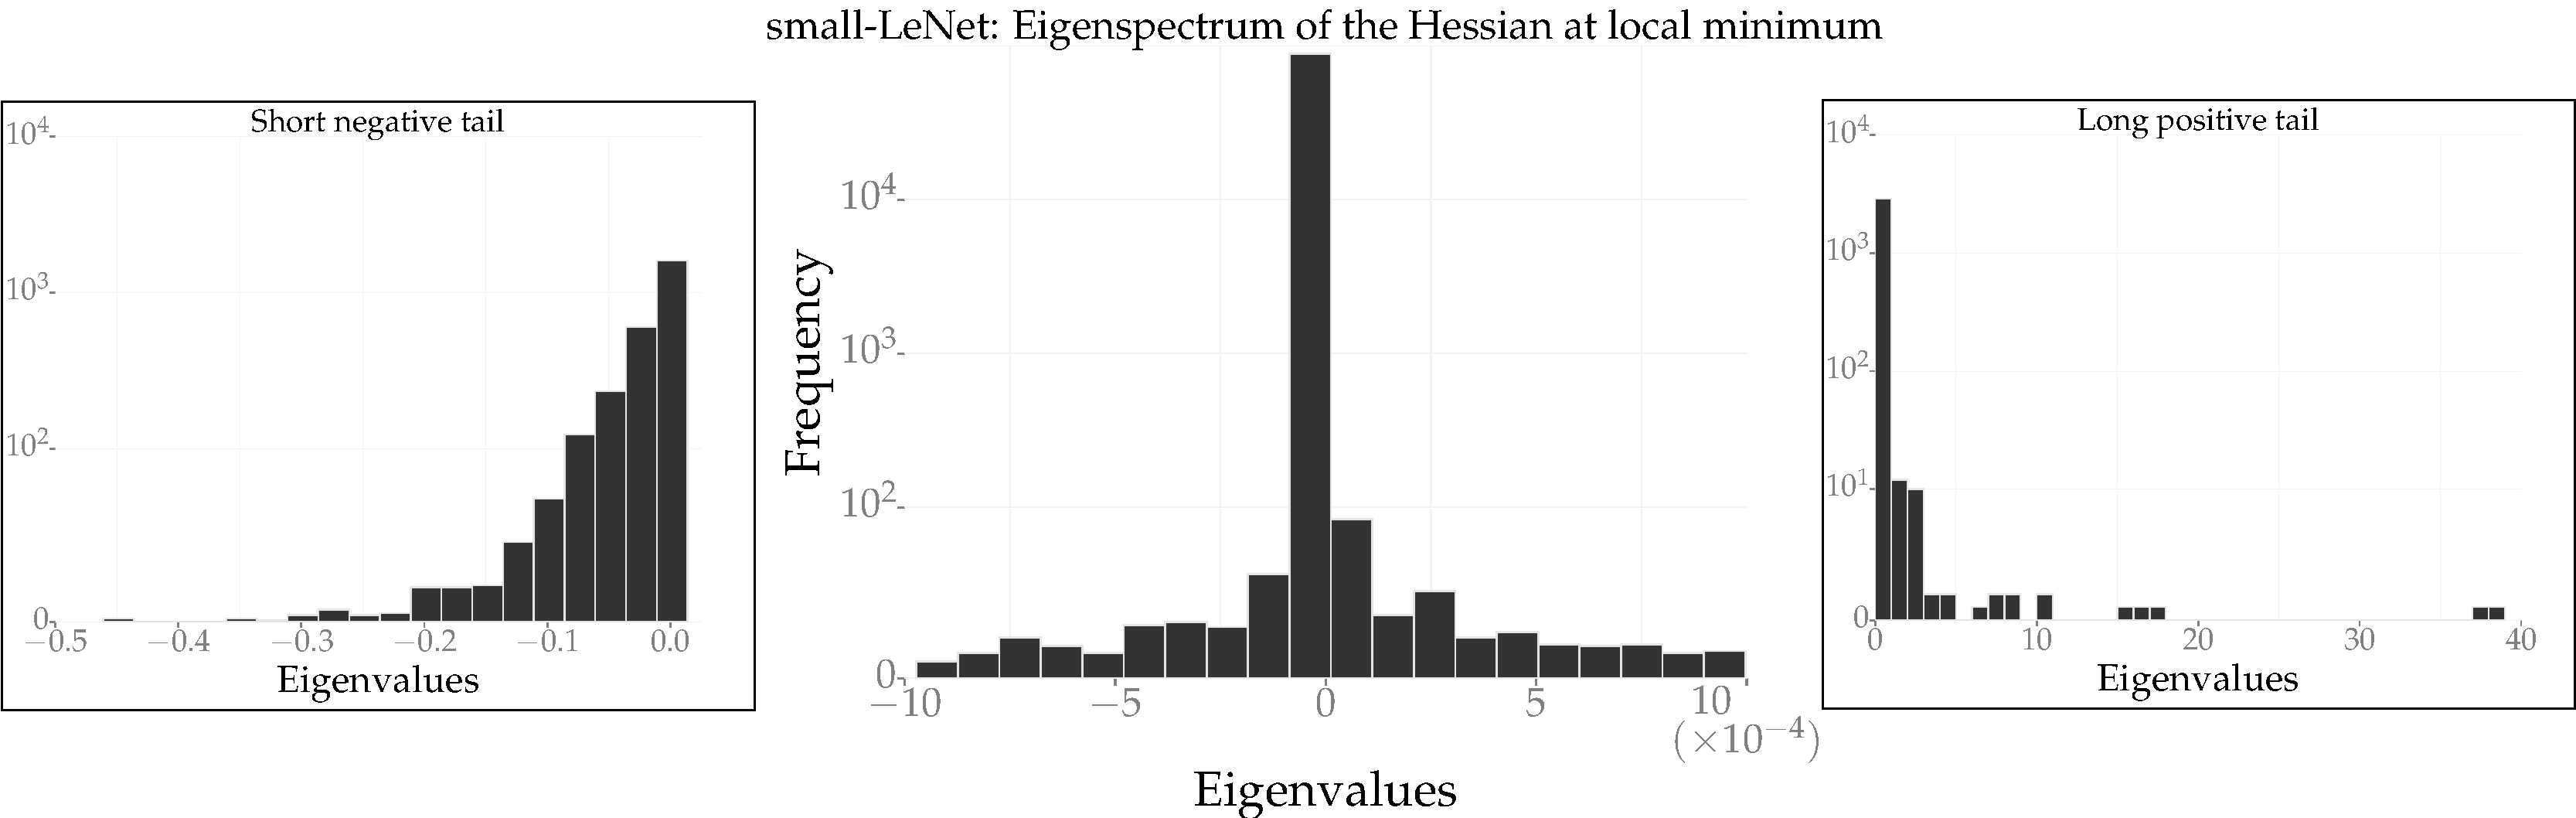
\includegraphics[width=\textwidth]{lenet_hessian.pdf}
\caption{\small Eigenspectrum of the Hessian at a local minimum of a CNN on MNIST (two independent runs). \textbf{Remark:} The central plot shows the eigenvalues in a small neighborhood of zero whereas the left and right insets show the entire tails of the eigenspectrum.}
\label{fig:lenet_hessian}
\end{figure}

Based on this understanding of how the local geometry looks at the end of optimization, can we modify SGD to actively seek such regions? Motivated by the work of~\citet{baldassi2015subdominant} on shallow networks, we propose to replace the original loss function $f(x)$ by:
$$
F(x, \g) = - \log \int_{x' \in \reals^n}\ \exp \rbrac{-f(x') - \f{\g}{2}\ \norm{x-x'}^2_2}\ dx'.
$$
The above is a log-partition function measures both the depth of a valley at a location  $x \in \reals^n$, and its flatness through the entropy of $f(x')$; we call it ``local entropy'' in analogy to the free entropy used in statistical physics. The $\entropysgd$ algorithm presented in this paper employs stochastic gradient Langevin dynamics (SGLD) to approximate the gradient of local entropy. Our algorithm resembles two nested loops of SGD: the inner loop consists of SGLD iterations while the outer loop updates the parameters. We show that the above modified loss function results in a smoother energy landscape defined by the hyper-parameter $\g$ which we can think of as a ``scope'' that seeks out valleys of specific widths. Actively biasing the optimization towards wide valleys in the energy landscape results in better generalization error. We present experimental results on fully-connected and convolutional neural networks (CNNs) on the MNIST and CIFAR-10~\citep{krizhevsky2009learning} datasets and recurrent neural networks (RNNs) on the Penn Tree Bank dataset (PTB)~\citep{marcus1993building} and character-level text prediction. Our experiments show that $\entropysgd$ scales to deep networks used in practice, obtains comparable generalization error as competitive baselines and also trains much more quickly than SGD.

\section{Related work}
\label{s:prior_work}

Our above observation about the spectrum of Hessian (further discussed in Sec.~\ref{s:expt}) is similar to results on a perceptron model in~\citet{dauphin2014identifying} where the authors connect the loss function of a deep network to a high-dimensional Gaussian random field. They also relate to earlier studies such as~\citet{Baldi:1989:NNP:70359.70362,Fyodorov2007,Bray2007} which show that critical points with high training error are exponentially likely to be saddle points with many negative directions and all local minima are likely to have error that is very close to that of the global minimum. The authors also argue that convergence of gradient descent is affected by the proliferation of saddle points surrounded by high error plateaus --- as opposed to multiple local minima. One can also see this via an application of Kramer's law: the time spent by diffusion is inversely proportional to the smallest negative eigenvalue of the Hessian at a saddle point~\citep{bovier2006metastability}.

The existence of multiple, almost equivalent, local minima in deep networks has been predicted using a wide variety of theoretical analyses and empirical observations, e.g., papers such as~\citet{spinglass2015,DBLP:conf/colt/ChoromanskaLA15,chaudhari2015trivializing} that build upon results from statistical physics as also others such as~\citet{haeffele2015global} and~\citet{janzamin2015beating} that obtain similar results for matrix and tensor factorization problems. Although assumptions in these works are somewhat unrealistic in the context of deep networks used in practice, similar results are also true for linear networks which afford a more thorough analytical treatment~\citep{DBLP:journals/corr/SaxeMG13}. For instance,~\citet{soudry2016no} show that with mild over-parameterization and dropout-like noise, training error for a neural network with one hidden layer and piece-wise linear activation is zero at every local minimum. All these results suggest that the energy landscape of deep neural networks should be easy to optimize and they more or less hold in practice --- it is easy to optimize a prototypical deep network to near-zero loss \emph{on the training set}~\citep{hardt2015train,DBLP:journals/corr/GoodfellowV14}.
%Works such as which shows that for deep linear networks with more than three layers, there exist ``bad'' saddle points, i.e., where the Hessian has no negative eigenvalues; SGD will find it difficult to make progress in such regions.

Obtaining good \emph{generalization} error, however, is challenging: complex architectures are sensitive to initial conditions and learning rates~\citep{sutskever2013importance} and even linear networks~\citep{kawaguchi2016deep} may have degenerate and hard to escape saddle points~\citep{ge2015escaping,anandkumar2016efficient}. Techniques such as adaptive~\citep{duchi2011adaptive} and annealed learning rates, momentum~\citep{tieleman2012lecture}, as well as architectural modifications like dropout~\citep{srivastava2014dropout}, batch-normalization~\citep{ioffe2015batch,cooijmans2016recurrent}, weight scaling~\citep{salimans2016weight} etc. are different ways of tackling this issue by making the underlying landscape more amenable to first-order algorithms. However, the training process often requires a combination of such techniques and it is unclear beforehand to what extent each one of them helps.

\todo{Closer to the subject of this paper are results by~\citet{baldassi2015subdominant,baldassi2016unreasonable,baldassi2016multilevel} which show that the energy landscape of shallow networks with discrete weights is characterized by an exponential number of isolated minima and few very dense regions with lots of local minima close to each other. These dense local minima can be shown to generalize well for random input data; more importantly, they are also accessible by efficient algorithms using a novel measure called ``robust ensemble'' that amplifies the weight of such dense regions. Algorithms 

Let us note that a related work in this direction is EASGD~\citep{zhang2015deep} which trains multiple deep networks in parallel and modulates the distance of each worker to the ensemble average. An ensemble training procedure provides improved generalization by ensuring that different works land in the same wide valley and indeed, this turns out to be closely related to the robust ensemble approach.
%
Our work generalizes the local entropy approach to modern deep networks with continuous weights. It exploits the same phenomenon of wide valleys in the energy landscape but does so without incurring the hardware and communication complexity of a distributed training algorithm.}

The authors in~\citet{hochreiter1997flat} introduce hard constraints on the width of local minima and training loss and show using the Gibbs formalism~\citep{haussler1997mutual} that this leads to improved generalization. \pc{Their analysis of the generalization performance (see their Sec. A1) necessitates a few unrealistic assumptions whereas in our analysis, as will be shown, we use uniform stability~\citet{bousquet2002stability} to obtain a precise characterization of generalization.}{} Furthermore, as they mention, the effect of hyper-parameters for the constraints they use is intricately tied together and they are difficult to choose even for small problems. Their formulation depends on Hessian-vector products. It is unclear how this method could be scaled to modern deep networks. Motivated by the same final goal, viz., flat local minima, our approach eliminates these extraneous and difficult to control hyper-parameters and instead results in a scalable algorithm. Also recent work by~\citet{keskar2016large} is relevant in the context of the main theme of our paper. The authors estimate the loss in a neighborhood of the weights to argue that small batch size in SGD (i.e., larger gradient noise) generalizes better than large mini-batches and also results in significantly flatter minima.

In the sense that local entropy results in a smoother energy landscape (cf.\@ Sec.~\ref{ss:theoretical_properties}), it resembles continuation methods~\citep{allgower2012numerical} that convolve the loss function to solve sequentially refined optimization problems. These techniques however require a special class of loss functions where successively smaller convolutions result in minimizers that lie close to each other or closed-form expressions of smoothened loss functions~\citep{,DBLP:conf/icml/HazanLS16,mobahi2015link}; these may not be possible for deep networks with isolated minima and highly-nonlinear loss functions. Our modified objective instead weighs each location by the local entropy in its neighborhood and does not require stringent assumptions on the objective, it is also applicable to full-scale deep networks. %\pc{Let us also note that motivated from continuation,~\citet{gulcehre2016mollifying} insert annealed additive noise in the activation function to approximately convolve the original objective function.}{This paper is not related to our work, it is related to continuation. I don't see any reason to add this sentence}

\section{Local entropy}
\label{s:local_entropy}

We first provide a simple intuition for the concept of local entropy of an energy landscape. Consider a cartoon energy landscape in Fig.~\ref{fig:entropyfig} where the x-axis denotes the configuration space of the parameters. We have constructed two local minima: a shallower although wider one at $x_{\trm{robust}}$ and a very sharp global minimum at $x_{\trm{non-robust}}$. Under a Bayesian prior on the parameters, say a Gaussian of a fixed variance at locations $x_{\trm{robust}}$ and $x_{\trm{non-robust}}$ respectively, the wider local minimum has a higher marginalized likelihood than the sharp valley on the right.

\begin{wrapfigure}{r}{0.4\textwidth}
\centering
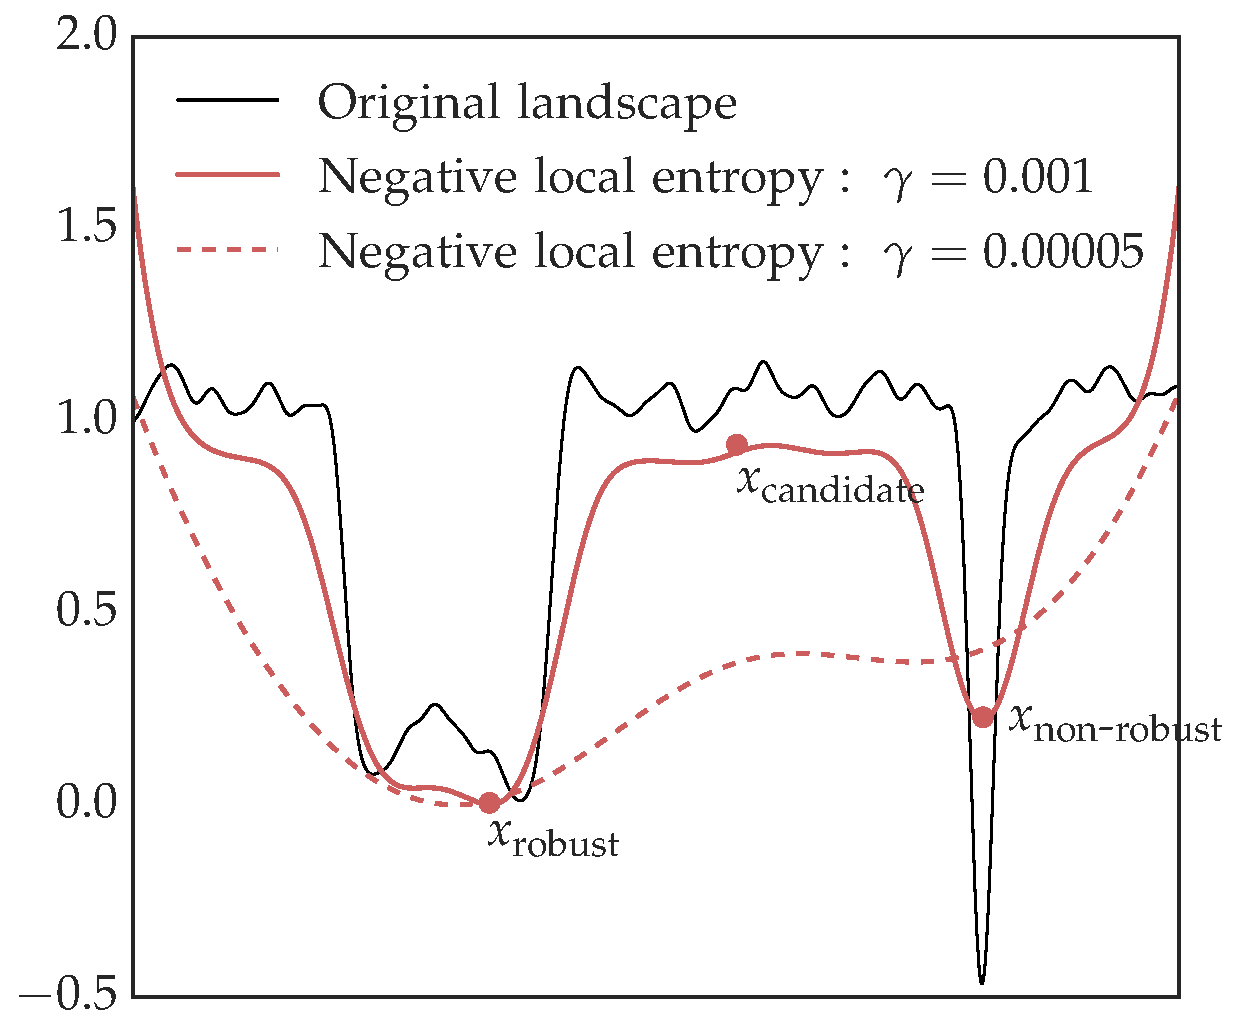
\includegraphics[width=0.4 \textwidth]{entropyfig.pdf}
\caption{\small Local entropy concentrates on wide valleys in the energy landscape.}
\label{fig:entropyfig}
\vspace*{-0.1in}
\end{wrapfigure}

The above discussion suggests that parameters that lie in wider local minima like $x_{\trm{robust}}$, which may possibly have a higher loss than the global minimum, should generalize better than the ones that are simply at the global minimum. In a neighborhood of $x_{\trm{robust}}$, ``local entropy'' as introduced in Sec.~\ref{s:intro} is large because it includes the contributions from a large region of good parameters; conversely, near $x_{\trm{non-robust}}$, there are fewer such contributions and the resulting local entropy is low. The local entropy thus provides a way of picking large, approximately flat, regions of the landscape over sharp, narrow valleys in spite of the latter possibly having a lower loss. Quite conveniently, the local entropy is also computed from the partition function with a local re-weighting term.

Formally, for a parameter vector $x \in \reals^n$, consider a Gibbs distribution corresponding to a given energy landscape $f(x)$:
\begin{equation}
    \P(x;\ \b) = Z_\b^{-1}\ \exp\ \rbrac{-\b\ f(x)};
    \label{eq:gibbs_original}
\end{equation}
where $\b$ is known as the inverse temperature and $Z_\b$ is a normalizing constant, also known 
as the partition function. As $\b \to \infty$, the probability distribution above concentrates on the global minimum of $f(x)$ (assuming it is unique) given as:
\begin{equation}
    x^* = \argmin_x\ f(x),
    \label{eq:argmin_generic}
\end{equation}
which establishes the link between the Gibbs distribution and a generic optimization problem~\eqref{eq:argmin_generic}. We would instead like the probability distribution --- and therefore the underlying optimization problem --- to focus on flat regions such as $x_{\textrm{robust}}$ in Fig.~\ref{fig:entropyfig}. With this in mind, let us construct a modified Gibbs distribution:
\begin{equation}
    \P(x';\ x, \b, \g) = Z_{x,\b,\ \g}^{-1}\ \exp\ \rbrac{-\b\ f(x') - \b\ \f{\g}{2}\ \norm{x-x'}^2_2}.
    \label{eq:gibbs_modified}
\end{equation}
The distribution in~\eqref{eq:gibbs_modified} is a function of a dummy variable $x'$ and is parameterized by the original location $x$. The parameter $\g$ biases the modified distribution~\eqref{eq:gibbs_modified} towards $x$; a large $\g$ results in a $P(x';\ x,\b,\g)$ with all its mass near $x$ irrespective of the energy term $f(x')$. For small values of $\g$, the term $f(x')$ in the exponent dominates and the modified distribution is similar to the original Gibbs distribution in~\eqref{eq:gibbs_original}. We will set the inverse temperature $\b$ to $1$ because $\g$ affords us similar control on the Gibbs distribution.

\begin{definition}[Local entropy]
\label{def:local_entropy}
The local free entropy of the Gibbs distribution in~\eqref{eq:gibbs_original}, colloquially called ``local entropy'' in the sequel and denoted by $F(x, \g)$, is defined as the log-partition function of modified Gibbs distribution~\eqref{eq:gibbs_modified}, i.e.,
\begin{align}
    F(x, \g) &= \log Z_{x, 1, \g} \notag\\
    &= \log \int_{x'}\ \exp \Big(-f(x') - \f{\g}{2}\ \norm{x-x'}^2_2 \Big)\ dx'.
    \label{eq:local_entropy}
\end{align}
\end{definition}
The parameter $\g$ is used to focus the modified Gibbs distribution upon a local neighborhood of $x$ and we call it a ``scope'' henceforth. Fig.~\ref{fig:entropyfig} shows the negative local entropy $-F(x, \g)$ for the original energy landscape. Note that $-F(x, \g)$ has a global minimum near $x_{\textrm{robust}}$ which is exactly what we want; indeed, $x_{\textrm{robust}}$ has a higher local entropy than $x_{\textrm{non-robust}}$.

\paragraph{Connection to classical entropy:}
The quantity we have defined as local entropy in Def.~\ref{def:local_entropy} is different from classical entropy which counts the number of likely configurations under a given distribution. For a continuous parameter space, this is given by
$$
    S(x, \b, \g) = - \int_{x'}\ \log \P(x';\ x, \b, \g)\ d \P(x';\ x, \b, \g)
$$
for the Gibbs distribution in~\eqref{eq:gibbs_modified}. Minimizing classical entropy however does not differentiate between flat regions that have very high loss versus dense regions that lie deeper in the energy landscape. For instance, in Fig.~\ref{fig:entropyfig}, classical entropy is smallest in the neighborhood of $x_{\textrm{candidate}}$ which is a large region with very high loss on the training dataset and is unlikely to generalize well.
\ignore{We could minimize a modified loss function of the form $f(x) + \lambda S(x, \g)$ whose gradient can be computed to be
$$
    \nabla \Big(f(x) + \lambda S(x, \g)\Big) = \nabla f(x) - \lambda \g\ \corr (g(x'),\ x-x');
$$
where we have defined the cross-correlation as
$$
    \corr (g(x'),\ x-x') := \ag{g(x')\ (x-x')} - \ag{g(x')}\ \ag{x-x'};
$$
with $g(x') = f(x') + \f{\g}{2}\ \norm{x-x'}^2_2$. The gradient of the entropy can again be estimated using Langevin dynamics. Practically, one then has to modulate the hyper-parameter $\lambda$ during the course of the training to first use the gradient $\nabla f(x)$ to make progress and then turn on the entropy term to scope dense clusters.}

\section{Entropy-guided SGD}
\label{s:entropysgd}

We now present the $\entropysgd$ algorithm that is a variation of SGD motivated from local entropy. Simply speaking, it minimizes the negative local entropy from Sec.~\ref{s:local_entropy}. This section discusses how the gradient of local entropy can be computed via Langevin dynamics; the resulting algorithm has a strong flavor of ``SGD-inside-SGD'': the outer SGD updates the parameters, while an inner SGD estimates the gradient of local entropy.

Consider a typical classification setting, let $x \in \reals^n$ be the weights of a deep neural network and $\xi_k \in \Xi$ be samples from a dataset $\Xi$ of size $N$. Let $f(x; \xi_k)$ be the loss function, e.g., cross-entropy of the classifier on a sample $\xi_k$. The original optimization problem is:
\begin{equation}
    x^* = \argmin_x\ \f{1}{N}\ \sum_{k=1}^N\ f(x;\ \xi_k);
    \label{eq:dnn_objective}
\end{equation}
where the objective $f(x, \xi_k)$ is typically, a non-convex function in both the weights $x$ and the sample $\xi_k$. The $\entropysgd$ algorithm instead solves the problem
\begin{equation}
    x^*_{\entropysgd} = \argmin_x\ -F(x, \gamma;\ \Xi);
    \label{eq:entropysgd_objective}
\end{equation}
where we have made the dependence of local entropy $F(x,\g)$ on the dataset $\Xi$ explicit.

\subsection{Gradient of local entropy}
\label{ss:grad_local_entropy}

The gradient of local entropy over a randomly sampled mini-batch of $m$ samples denoted by $\xi_{\ell_i} \in \minibatch{\ell}$ for $i \leq m$ is easy to derive and is given by
\begin{equation}
    -\nabla_x F\rbrac{x, \g;\ \minibatch{\ell}} = \g\ \rbrac{x - \ag{x';\ \minibatch{\ell}}};
    \label{eq:entropysgd_grad}
\end{equation}
where the notation $\ag{\cdot}$ denotes an expectation of its arguments (we have again made the dependence on the data explicit) over a Gibbs distribution of the original optimization problem modified to focus on the neighborhood of $x$; this is given by
\begin{equation}
    \P(x';\ x, \g) \propto\ \exp \sqbrac{-\rbrac{\f{1}{m}\ \sum_{i=1}^m\ f\rbrac{x;\ \xi_{\ell_i}}} - \f{\g}{2}\ \norm{x-x'}_2^2}.
    \label{eq:entropysgd_modified_gibbs}
\end{equation}
Computationally, the gradient in~\eqref{eq:entropysgd_grad} involves estimating $\ag{x';\ \minibatch{\ell}}$ with the current weights fixed to $x$. This is an expectation over a Gibbs distribution and is hard to compute. We can however approximate it using Markov chain Monte-Carlo (MCMC) techniques. In this paper, we use stochastic gradient Langevin dynamics (SGLD)~\citep{welling2011bayesian} that is an MCMC algorithm for drawing samples from a Bayesian posterior and scales to large datasets using mini-batch updates. Please see Sec.~\ref{s:app:langevin} in the Supplement for a brief overview of SGLD. For our application, as lines 3-6 of Alg.~\ref{alg:entropysgd} show, SGLD resembles a few iterations of SGD with additive gradient noise.

We can obtain some intuition of how $\entropysgd$ works using the expression for the gradient: the term $\ag{x';\ \cdot}$ is the average over a locally focused Gibbs distribution and for two local minima in the neighborhood of $x$ roughly equivalent in loss, this term points towards the wider one because $\ag{x';\ \cdot}$ is closer to it. This results in a net gradient that takes SGD towards wider valleys. Moreover, if we unroll the SGLD steps used to compute $\rbrac{x - \ag{x'; \cdot}}$ (cf. line 5 in Alg.~\ref{alg:entropysgd}), it resembles one large step in the direction of the (noisy) average gradient around the current weights $x$ and $\entropysgd$ thus looks similar to averaged SGD in the literature~\citep{polyak1992acceleration,bottou2012stochastic}. These two phenomena intuitively explain the improved generalization performance of $\entropysgd$.

\subsection{Algorithm and Implementation details}
\label{ss:alg}

Alg.~\ref{alg:entropysgd} provides the pseudo-code for one iteration of the $\entropysgd$ algorithm. At each iteration, lines $3$-$6$ perform $L$ iterations of Langevin dynamics to estimate $\mu = \ag{x'; \minibatch{\ell}}$. The weights $x$ are updated with the modified gradient on line $9$.

\begin{center}
\begin{minipage}{0.7 \textwidth}
\IncMargin{0.04in}
\begin{algorithm}[H]
    \SetKwInOut{Input}{Input}
    \SetKwInOut{HyperParameters}{Hyper-parameters}

    \small
    \Input{\quad $\textrm{current weights}\ x$, $\textrm{Langevin iterations}\ L$}
    \HyperParameters{\quad $\textrm{Scope}\ \g$, $\textrm{Learning rate}\ \eta$}
    \vspace{0.1in}
    \nonl \textrm{// SGLD iterations}\;
    \vspace{0.025in}
    $x', \mu \la x$\;
    \For{$\ell \leq L$}
    {
        $\minibatch{\ell} \la \textrm{sample mini-batch}$\;
        \vspace{0.03in}
        $dx' \la \f{1}{m}\ \sum_{i=1}^m\ \nabla_{x'} f\rbrac{x';\ \xi_{\ell_i}} - \g\ \rbrac{x - x'}$\;
        \vspace{0.03in}
        $x' \la x' - \eta'\ dx' + \sqrt{\eta'}\ \trm{N}(0, \e\ \trm{I})$\;
        \vspace{0.03in}
        $\mu \la (1-\a) \mu + \a\ x'$\;
    }
    \vspace{0.1in}
    \nonl \textrm{// Update weights}\;
    \vspace{0.03in}
    $x \la x - \eta\ \g\ (x-\mu)$
    \caption{$\entropysgd$ algorithm}
    \label{alg:entropysgd}
\end{algorithm}
\DecMargin{0.04in}
\end{minipage}
\end{center}

\todo{
We set the number of SGLD iterations $L$ to $5$-$20$ depending upon the complexity of the dataset, e.g., for experiments on convolutional networks on MNIST and CIFAR-10, we use $L = 20$ while for experiments on a fully-connected network on MNIST $L=5$ works well (cf. Sec.~\ref{s:expt}). We perform exponential averaging of the Langevin iterates $x'$ to estimate $\mu$ with a parameter $\a = 0.9$ so as to put more weight on later samples. In order to quickly transition to the Langevin dynamics phase of SGLD and ensure the we are sampling from the posterior even for small values of $L$, we set the learning rate $\eta'$ on line $5$ to be small factor of the outer SGD's learning rate: $\eta' = 0.1\ \eta$~\citep{welling2011bayesian}.}

Let us note that although we have written Alg.~\ref{alg:entropysgd} in the classical SGD setup, we can easily modify it to include techniques such as momentum and gradient pre-conditioning~\citep{duchi2011adaptive} by changing lines $5$ and $9$. In our experiments, we have used both SGD with Nesterov's momentum~\citep{sutskever2013importance} and Adam for outer and inner loops with similar qualitative results.

\subsubsection{Scoping of $\gamma$}

\subsection{Connection to variational inference}
\label{ss:connection_variational}


\subsection{Theoretical Properties}
\label{ss:theoretical_properties}

\pc{We can show that $\entropysgd$ results in a smoother loss function and obtains better generalization error than the original objective~\eqref{eq:dnn_objective} if trained for the same number of iterations. Proofs are deferred to the Appendix (see Sec.~\ref{s:app:proofs}).}{Clarify that the analysis here is only a sketch, it is not rigorous}

With some overload of notation, we assume that the original loss $f(x)$ is $\b$-smooth, i.e., for all $x,y \in \reals^n$, we have $\norm{\nabla f(x) - \nabla f(y)} \leq \b\ \norm{x-y}$. We additionally assume for the purpose of analysis that no eigenvalue of the Hessian $\nabla^2 f(x)$ lies in the set $[-2 \g-c, c]$ for some small $c > 0$.
%
\begin{lemma}
\label{lem:smoothness_reduction}
The objective $F(x, \g;\ \Xi)$ in~\eqref{eq:entropysgd_objective} is $\f{\a}{1 + \g^{-1}\ c}$-Lipschitz and $\f{\b}{1 + \g^{-1}\ c}$-smooth.
\end{lemma}
The local entropy objective is thus smoother than the original objective while the modified objective in~\eqref{eq:entropysgd_objective} results in a factor of $\r + \f{1}{1 + \g^{-1}\ c}$ in the above lemma.

Let us now obtain a bound on the improvement in generalization error. We denote an optimization algorithm, viz., SGD or $\entropysgd$ by $A(\Xi)$, it is a function of the dataset $\Xi$ and outputs the parameters $x^*$ upon termination. Stability of the algorithm~\citep{bousquet2002stability} is then a notion of how much its output differs in loss upon being presented with two datasets $\Xi$ and $\Xi'$ that differ in at most one sample,
$$
    \sup_{\xi\ \in\ \Xi\ \cup\ \Xi'}\ \sqbrac{ f \rbrac{A(\Xi), \xi} - f \rbrac{A(\Xi'), \xi}} \leq \e.
$$
\citet{hardt2015train} connect uniform stability to generalization error and show that an $\e$-stable algorithm $A(\Xi)$ has generalization error bounded by $\e$, i.e., if $A(\Xi)$ terminates with parameters $x^*$,
$$
    \abs{ \E_{\Xi} \rbrac{R_\Xi(x^*) - R(x^*)} } \leq \e;
$$
where the left hand side is the generalization error: it is the difference between the empirical loss $R_\Xi(x) := \f{1}{N}\ \sum_{k=1}^N\ f(x, \xi_k)$ and the population loss $R(x) := \E_{\xi}\ f(x, \xi)$.

We now employ the following theorem that bounds the stability of an optimization algorithm through the smoothness of its loss function and the number of iterations on the training set.
\begin{theorem}[\citet{hardt2015train}]
\label{thm:generalization_bound_nonconvex}
For an $\a$-Lipschitz and $\b$-smooth loss function, if SGD converges in $T$ iterations on $N$ samples with decreasing learning rate $\eta_t \leq 1/t$ the stability is bounded by
\begin{align*}
    \e
    %&\leq \f{1}{N-1}\ \rbrac{1 + \f{1}{\b c}}\ \rbrac{2 c \a^2}^{\f{1}{1 + \b c}}\ T^{\f{\b c}{1 + \b c}}\\
    &\lessapprox \f{1}{N}\ \a^{1/(1 + \b)}\ T^{1 - 1/(1 + \b)}.
\end{align*}
\end{theorem}
%
Using Lem.~\ref{lem:smoothness_reduction} and Thm.~\ref{thm:generalization_bound_nonconvex} we have
\begin{equation}
    \e_{\ \entropysgd} \lessapprox \rbrac{\a\ T^{-1}}^{\rbrac{1 - \f{1}{1 + \g^{-1}c}}\ \b}\ \e_{\ \textrm{SGD}},
    \label{eq:stability_bound}
\end{equation}
which shows that $\entropysgd$ generalizes better than SGD for all $T > \a$.

As an aside, it is easy to see from the proof of Lem.~\ref{lem:smoothness_reduction} that for a convex loss function $f(x)$, adding the local entropy term does not change the minimizer of the original problem.

\section{Experiments}
\label{s:expt}

In Sec.~\ref{ss:expt:universality}, we discuss experiments that suggest that the characteristics of the energy landscape around local minimal accessible by SGD are universal to deep architectures.  This observation motivates the $\entropysgd$ algorithm considered in this paper and in Sec.~\ref{ss:expt:mnist} and~\ref{ss:expt:cifar}, we present experimental results on two standard image classification datasets, viz., MNIST and CIFAR-10.

\subsection{Universality of the Hessian at local minima}
\label{ss:expt:universality}

We use automatic differentiation\footnote{\href{https://github.com/HIPS/autograd}{https://github.com/HIPS/autograd}} to compute the Hessian at a local minimum obtained at the end of training for the following networks:

\begin{enumerate}[(i)]
\item \textbf{small-LeNet on MNIST}: This network has $47,658$ parameters and is similar to $\lenet$ but with $10$ and $20$ channels respectively in the first two convolutional layers and $128$ hidden units in the fully-connected layer. We train this with Adam to obtain a test error of $2.4\%$.
%
\item \textbf{small-$\mnistfc$ on MNIST}: A fully-connected network ($50,890$ parameters) with one layer of $32$ hidden units, ReLU non-linearities and cross-entropy loss; it converges to a test error of $2.5\%$ with momentum-based SGD.
%
\item \textbf{char-lstm for text generation}: This is a recurrent network with $48$ hidden units and Long Short-Term Memory (LSTM) architecture~\citep{hochreiter1997long}. It has $32,640$ parameters and we train it with Adam to re-generate a small piece of text consisting of $256$ lines of length $32$ each and $96$-bit one-hot encoded characters.
%
\item \textbf{$\allcnn$ on CIFAR-10}: This is similar to the All-CNN-C network~\citep{springenberg2014striving} with $\approx 1.6$ million weights (cf. Sec.~\ref{ss:expt:cifar}) which we train using Adam to obtain an error of $11.2\%$. Exact Hessian computation is in this case expensive and thus we instead compute the diagonal of the Fisher information matrix~\citep{wasserman2013all} using the element-wise first and second moments of the gradients that Adam maintains, i.e., $\trm{diag} (I) = \E(g^2) - (\E\ g)^2$ where $g$ is the back-propagated gradient. Fisher information measures the sensitivity of the log-likelihood of data given parameters in a neighborhood of a local minimum and thus is exactly equal to the Hessian of the negative log-likelihood. We will consider the diagonal of the empirical Fisher information matrix as a proxy for the eigenvalues of the Hessian, as is common in the literature.
\end{enumerate}

We choose to compute the exact Hessian and to keep the computational and memory requirements manageable, the first three networks considered above are smaller than standard deep networks used in practice. For the last network, we sacrifice the exact computation and instead approximate the Hessian of a large deep network. We note that recovering an approximate Hessian from Hessian-vector products~\citep{pearlmutter1994fast} could be a viable strategy for medium-scale networks.

Fig.~\ref{fig:lenet_hessian} in the introductory Sec.~\ref{s:intro} shows the eigenspectrum of the Hessian for small-LeNet while Fig.~\ref{fig:universality} shows the eigenspectra for the other three networks.
%
A large proportion of eigenvalues of the Hessian are very close to zero or positive with a very small (relative) magnitude. This is suggests that the local geometry of the energy landscape is almost flat at local minima discovered by gradient descent. This agrees with theoretical results such as~\citet{baldassi2016local} where the authors predict that flat regions of the landscape generalize better. Standard regularizers in deep learning such as convolutions, max-pooling and dropout seem to bias SGD towards flatter regions in the energy landscape.
%
The right tails of the eigenspectra are much longer than the left tails. Indeed, as discussed in numerous places in literature~\citep{Bray2007,dauphin2014identifying,spinglass2015}, SGD finds low-index critical points, i.e., optimizers with few negative eigenvalues of the Hessian. What is interesting and novel is that the directions of descent that SGD misses do not have a large curvature.

\begin{figure}[!tbh]
\centering
    \begin{subfigure}[t]{0.47 \textwidth}
        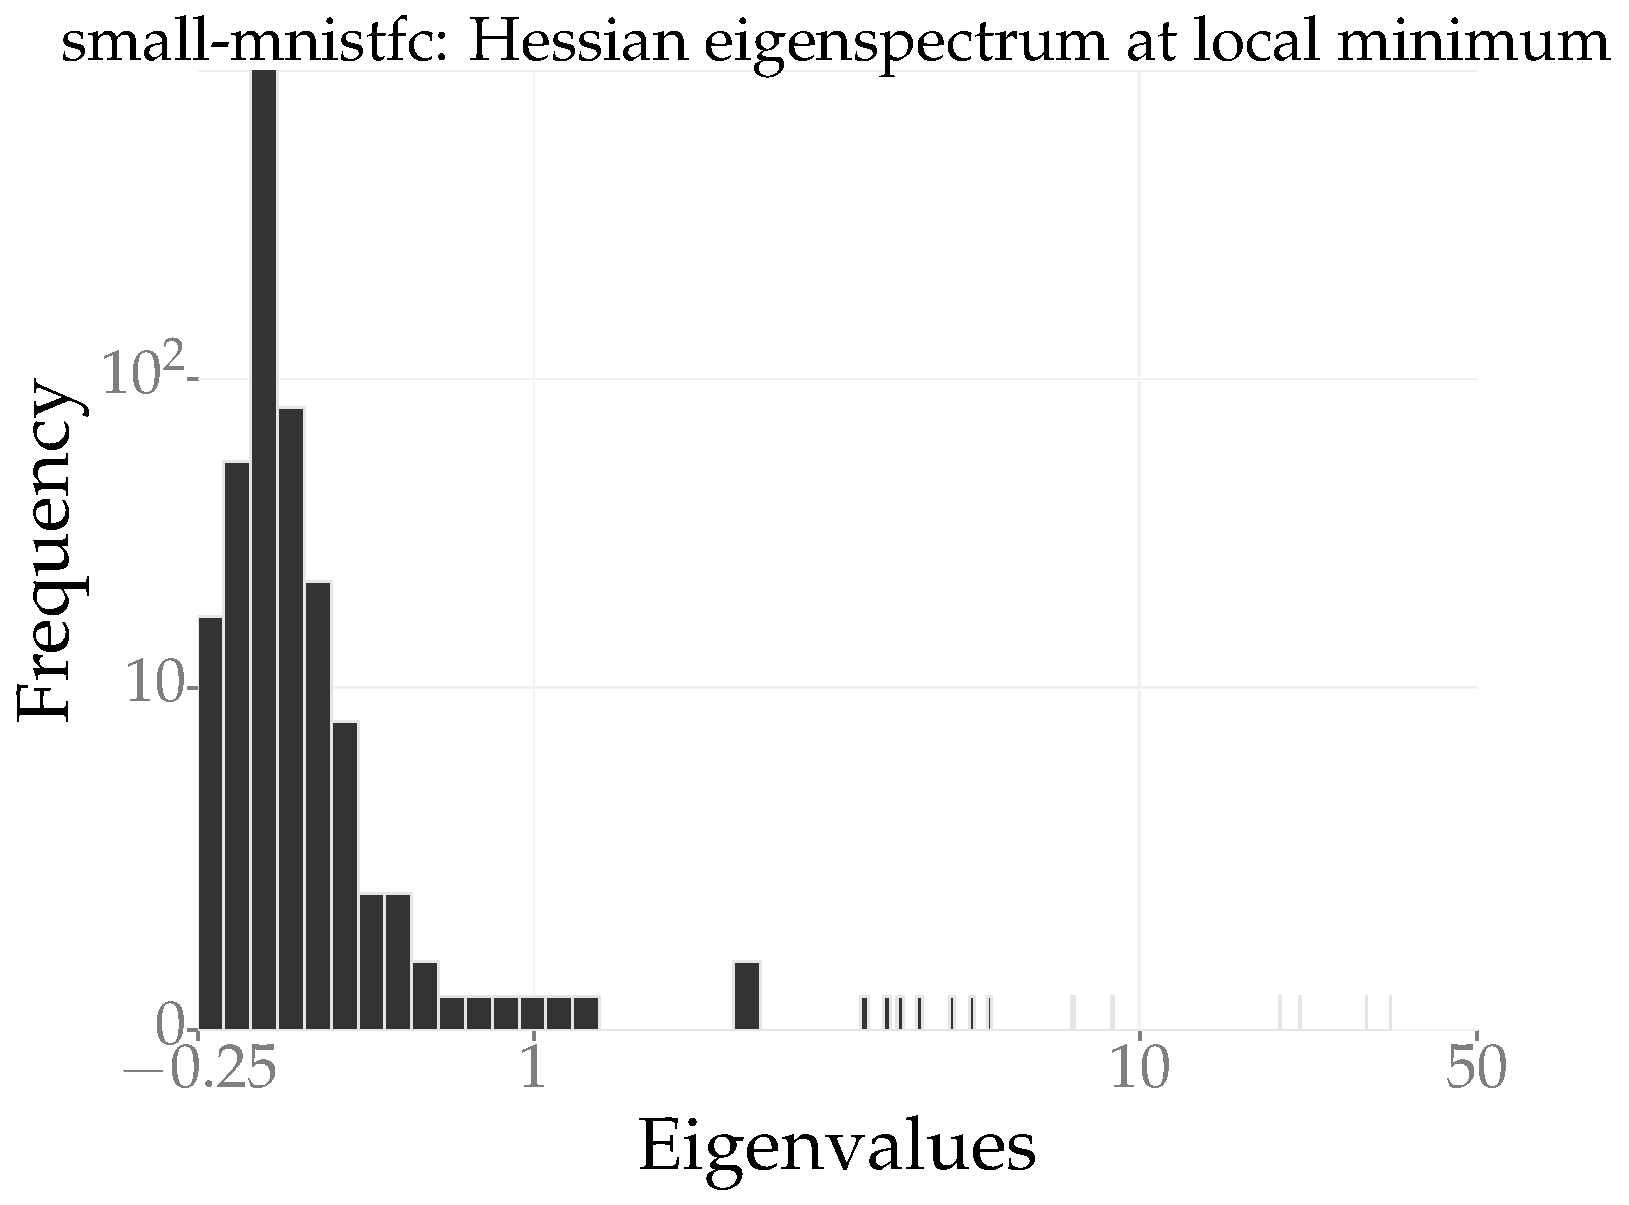
\includegraphics[width=1.08\textwidth]{mnistfc_hessian.pdf}
        \caption{\small $\smallmnistfc$ ($2$ runs): Peak (clipped here) at zero ($\abs{\lambda} \leq 10^{-2}$) accounts for $90\%$ of the entries.\vspace{0.15in}}
        \label{fig:mnistfc_hessian}
    \end{subfigure}
    \hspace{0.2in}
    \begin{subfigure}[t]{0.47 \textwidth}
        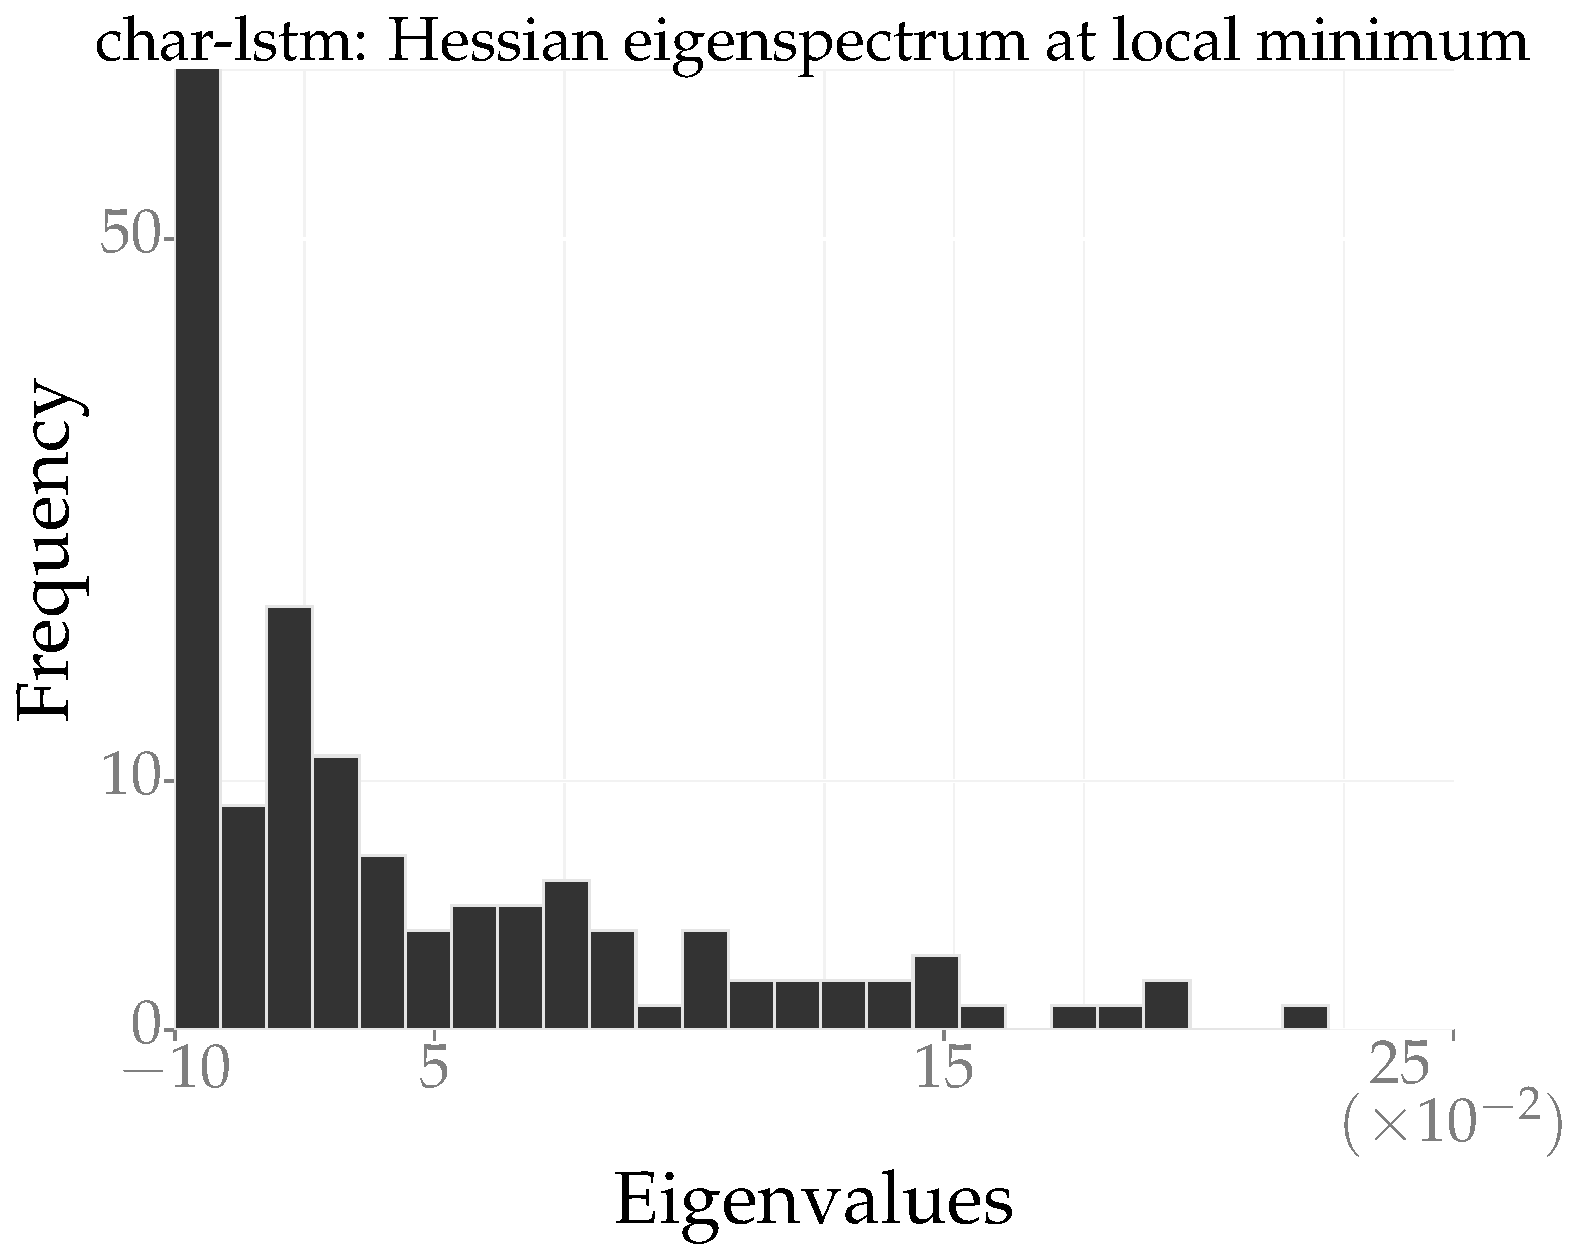
\includegraphics[width=\textwidth]{charlstm_hessian.pdf}
        \caption{\small $\charlstm$ ($5$ runs): Almost $95\%$ eigenvalues have absolute value below $10^{-5}$.}
        \label{fig:charlstm_hessian}
    \end{subfigure}
    \begin{subfigure}[b]{\textwidth}
        \centering
        \begin{subfigure}[b]{0.47 \textwidth}
        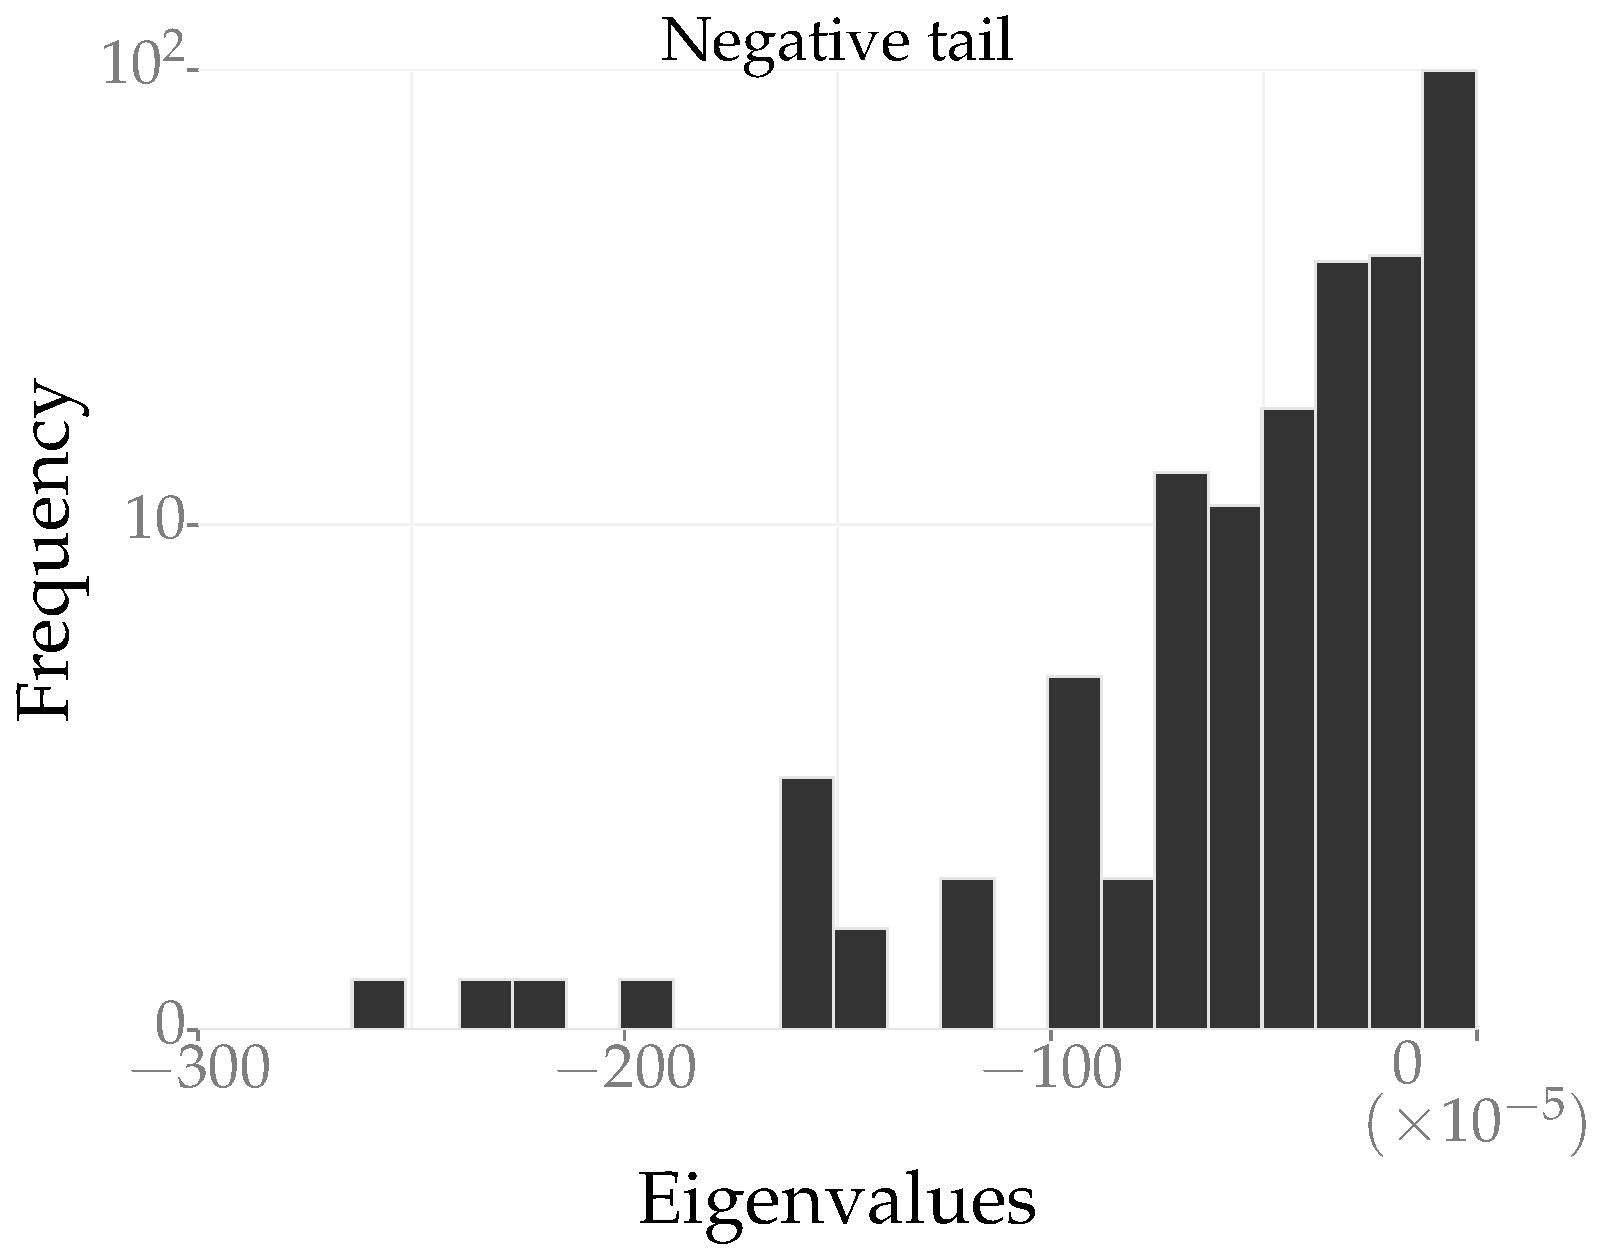
\includegraphics[width=\textwidth]{allcnn_dm.pdf}
        \end{subfigure}
        \hspace{0.2in}
        \begin{subfigure}[b]{0.47 \textwidth}
        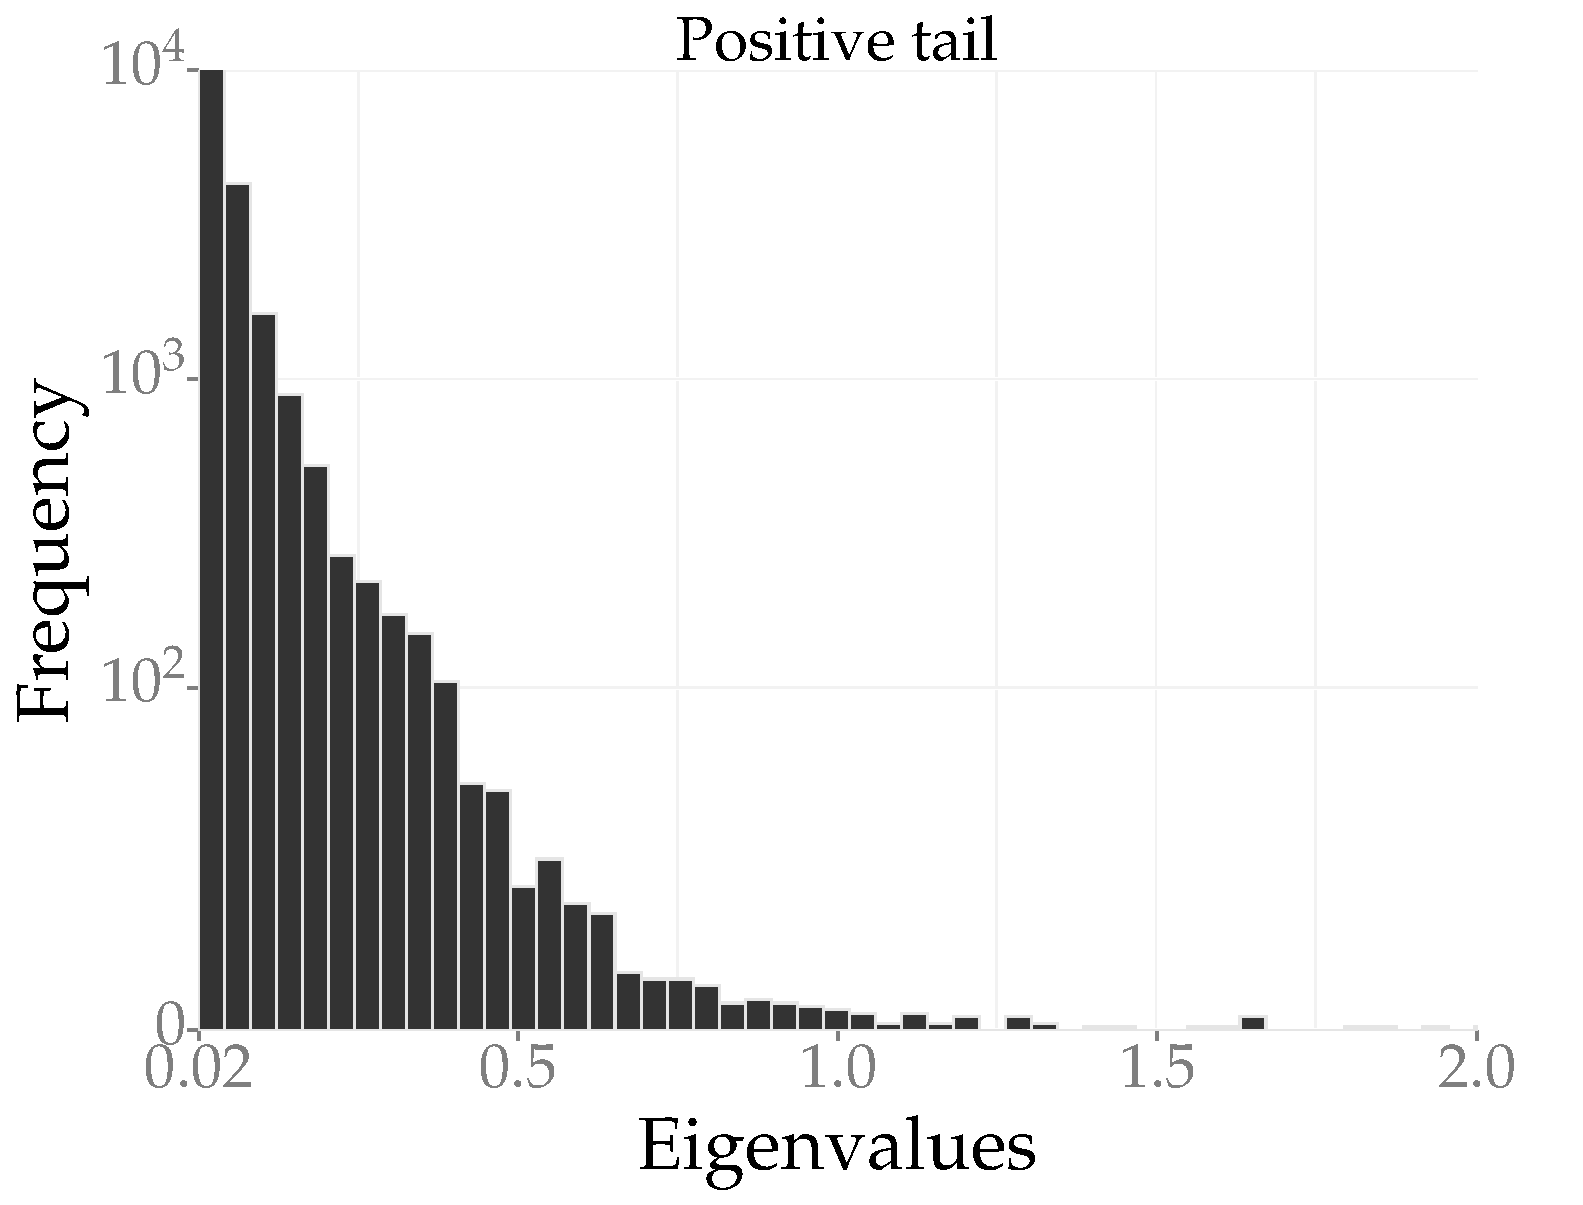
\includegraphics[width=\textwidth]{allcnn_dp.pdf}
        \end{subfigure}
    \caption{\small Negative and positive eigenvalues of the Fisher information matrix of $\allcnn$ at a local minimum ($4$ independent runs). The origin has a large peak with $\approx 95\%$ near-zero ($\abs{\lambda} \leq 10^{-5}$) eigenvalues (clipped here).}
    \label{fig:allcnn_hessian}
    \end{subfigure}
\caption{\small Universality of the Hessian: for a wide variety of network architectures, sizes and datasets, optima obtained by SGD are mostly flat (large peak near zero), they always have a few directions with large positive curvature (long positive tails). A very small fraction of directions have negative curvature, and the magnitude of this curvature is extremely small (short negative tails).}
\label{fig:universality}
\end{figure}

\subsection{MNIST}
\label{ss:expt:mnist}

In this section, we show that local entropy is a good measure of generalization, in fact, setting $\rho = 0$ in $\entropysgd$, i.e., completely disabling the original loss function is enough to train on MNIST. We consider two networks: the first is a fully-connected network with two hidden layers of $1024$ units each which we denote as ``$\mnistfc$'' and the second is a convolutional neural network similar to $\lenet$ but which batch-normalization~\citep{ioffe2015batch} and a dropout layer of probability $0.5$ added after each convolutional layer. We train for $100$ epochs with Adam and a learning rate of $10^{-3}$ that drops by a factor of $5$ after every $30$ epochs and compare the average error over $5$ independent runs in Fig.~\ref{fig:mnistfc_test} and Fig.~\ref{fig:lenet_test}.

$\entropysgd$ converges to an error of $1.39\%$ in $22$ epochs on $\mnistfc$ while Adam obtains the same (best) error after $67$ epochs. For a small network such as this, with a presumably easy energy landscape, we perform $5$ SGLD iterations and set $\g = 1$. For $\lenet$, we perform $20$ SGLD iterations and set $\g = 0.1$. In this case, $\entropysgd$ converges around epoch $40$ to an average error of $0.48\%$; Adam obtains a comparable error of $0.51\%$ after $100$ epochs. For this experiment, we use a small $\rho = 10^{-4}$ to fine-tune the network; the error without this is $0.52\%$.

\textbf{Remark:} A single ``epoch'' for all algorithms considered here corresponds to the number of parameter updates necessary to run through the entire dataset once. Note that both SGD and $\entropysgd$ update parameters after each mini-batch, but $\entropysgd$ also runs $L$ iterations of SGLD between two updates of the parameters.

\begin{figure}[h!]
\centering
    \begin{subfigure}[t]{0.45\textwidth}
        \centering
        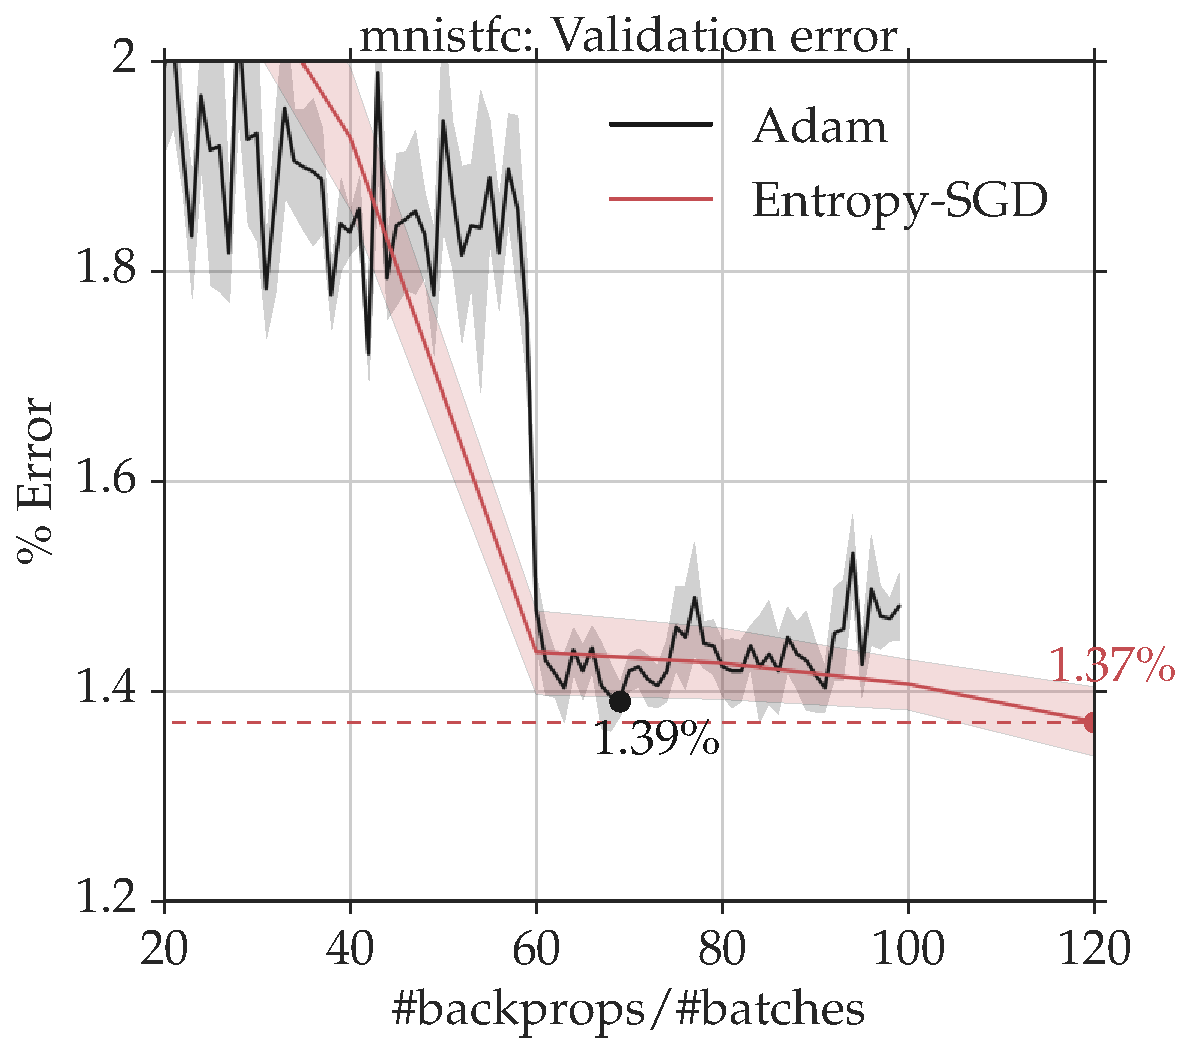
\includegraphics[width=0.98\textwidth]{mnistfc_valid.pdf}
        \caption{\small $\mnistfc$: $\entropysgd$ with $\rho = 0$, $L = 5$.}
        \label{fig:mnistfc_test}
    \end{subfigure}
    \hspace{0.1in}
    \begin{subfigure}[t]{0.45\textwidth}
        \centering
        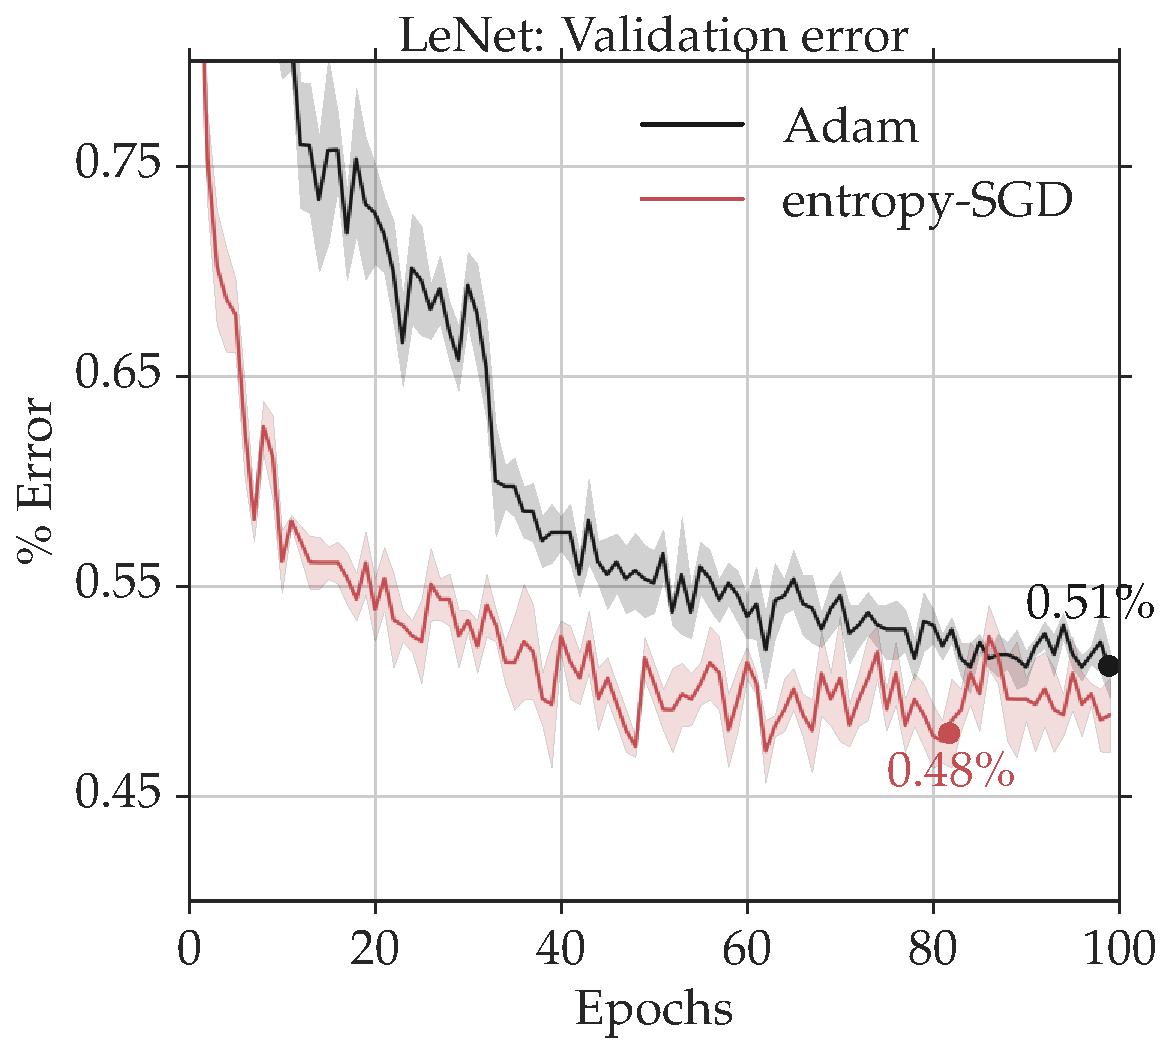
\includegraphics[width=\textwidth]{lenet_valid.pdf}
        \caption{\small $\lenet$: $\entropysgd$ $\rho = 10^{-4}$, $L = 20$.}
        \label{fig:lenet_test}
    \end{subfigure}
\caption{\small Comparison of $\entropysgd$ vs. Adam on MNIST\vspace*{0.15in}}
\label{fig:mnist_test}
\end{figure}

\begin{figure}[htp!]
\centering
    \begin{subfigure}[b]{0.45\textwidth}
        \centering
        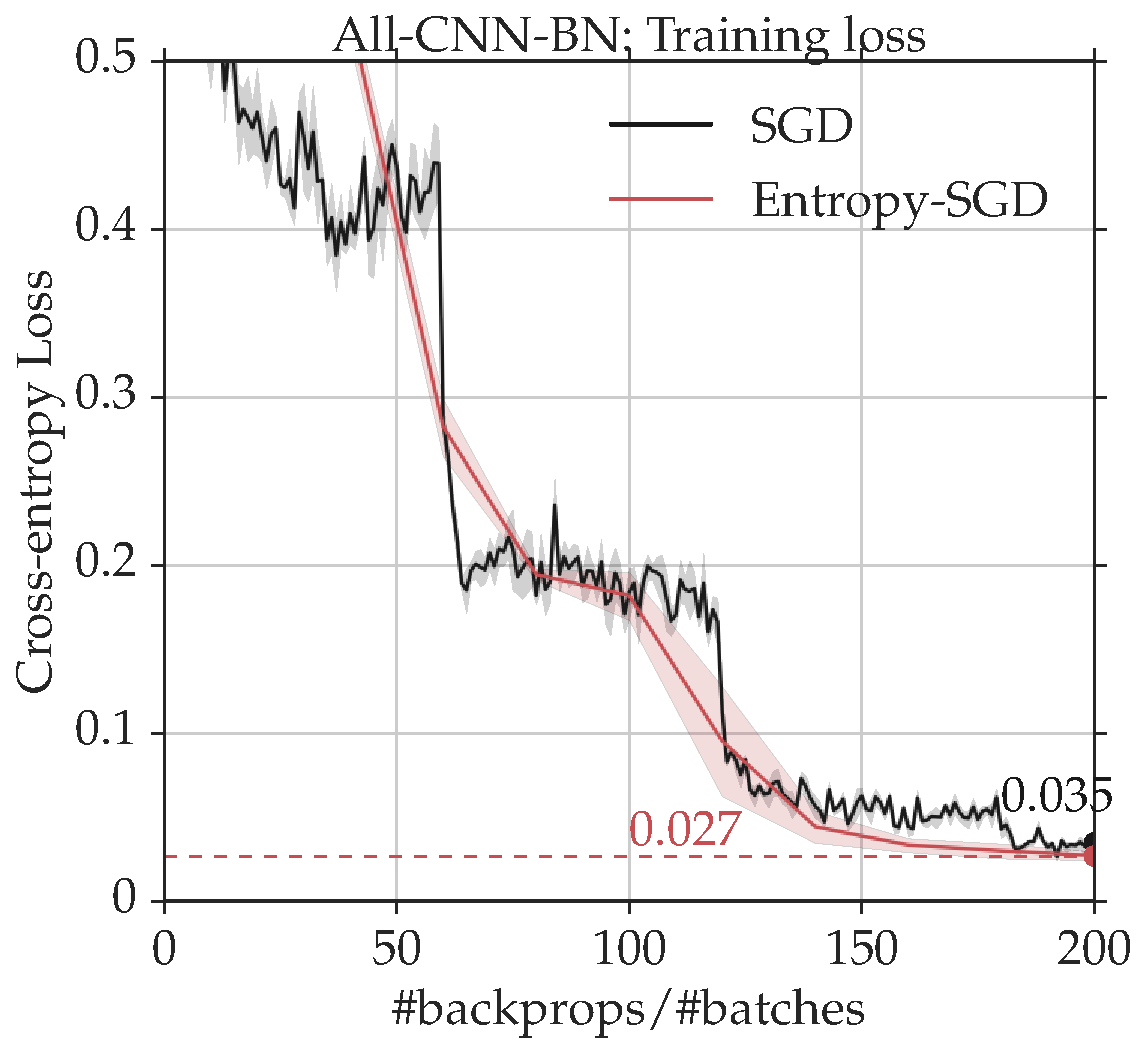
\includegraphics[width=1.03\textwidth]{allcnn_loss.pdf}
        \caption{\small $\allcnn$: Training loss}
        \label{fig:allcnn_loss}
    \end{subfigure}
    \hspace{0.1in}
    \begin{subfigure}[b]{0.45\textwidth}
        \centering
        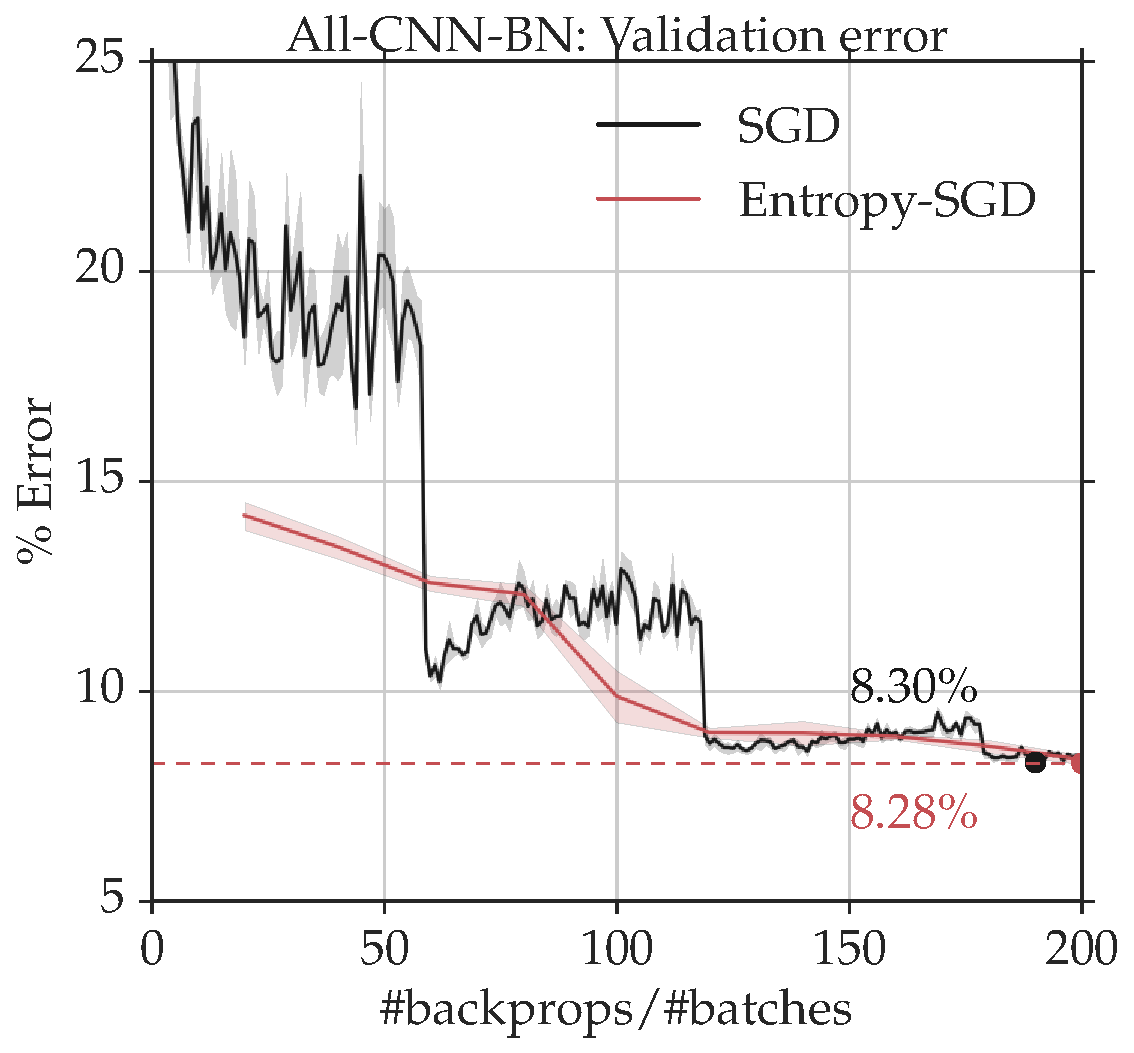
\includegraphics[width=\textwidth]{allcnn_valid.pdf}
        \caption{\small $\allcnn$: Validation error}
        \label{fig:allcnn_valid}
    \end{subfigure}
\caption{\small Comparison of $\entropysgd$ vs. Adam on CIFAR-10}
\label{fig:allcnn}
\end{figure}

\subsection{CIFAR-10}
\label{ss:expt:cifar}

We train on CIFAR-10 without data augmentation after performing global contrast normalization and ZCA whitening~\citep{goodfellow2013maxout}. As a baseline, we consider the All-CNN-C network of~\citet{springenberg2014striving} with a batch normalization layer after each convolutional layer; this is absent in the original paper. We recreate the training pipeline of the original authors with the same hyper-parameters and use SGD with Nesterov's momentum. We however decrease the initial learning rate of $0.1$ by a factor of $5$ after every $60$ epochs for SGD and after every $5$ epochs for $\entropysgd$. Probably due to batch-normalization, we obtain an average error of $8.30\%$ over $5$ runs of $200$ epochs vs.\ $9.08\%$ error in $350$ epochs as the authors in~\citet{springenberg2014striving} report. This gives us a very competitive baseline to compare $\entropysgd$ against. Let us note that the best result in literature on non-augmented CIFAR-10 is the ELU-network by~\citet{clevert2015fast} with $6.55\%$ test error while a wide ResNet of~\citet{zagoruyko2016wide} obtains an error of $4.17\%$ with data augmentation.

%We list a few other comparable networks in the literature in Table~\ref{tab:cifar10}.
% \begin{wraptable}{r}{0.6 \textwidth}
% \centering
% \renewcommand{\arraystretch}{1.2}
% \resizebox{0.5 \columnwidth}{!}
% {
% \begin{tabular}{p{6.5cm} r}
%     Model & Test error ($\%$)\\  \hline
%     %Maxout~\citep{goodfellow2013maxout} & $11.68$\\
%     NiN~\citep{lincy13} & $10.41$\\
%     All-CNN-C~\citep{springenberg2014striving} & $9.04$\\
%     All-CNN-BN (baseline: SGD, 200 epochs) & $8.30\ \pm\ 0.08$\\
%     All-CNN-BN ($\entropysgd$, 15 epochs) & $8.65\ \pm\ 0.06$\\
%     ELU~\citep{clevert2015fast} & $6.55$\\ \hline
% \end{tabular}
% }
% \caption{\small Error rates on CIFAR-10 without data augmentation.}
% \label{tab:cifar10}
% \end{wraptable}

Fig.~\ref{fig:allcnn} compares $\entropysgd$ against SGD with $20$ SGLD iterations for $15$ epochs. Since CIFAR-10 is a more challenging dataset than MNIST, we could not obtain better test errors than $9.5\%$ while training with only the local entropy term ($\rho = 0$). We therefore set $\rho = 0.01$ to obtain an error of $8.65\%$ over $5$ independent runs. Refer to Fig.~\ref{fig:allcnn_loss}, $\entropysgd$ is designed to be an algorithm that seeks out wide local minima as opposed to sharp valleys; a side-effect of this is to smooth the energy landscape as we show in Sec.~\ref{ss:theoretical_properties}. In practice, we see this as a steady decrease in training loss for $\entropysgd$ without any plateaus that appear in the training loss for SGD. Similarly, the decrease in validation error in Fig.~\ref{fig:allcnn_valid} is also steady without any plateaus. Note that the original network $\textrm{All-CNN-C}$ was trained using SGD for $350$ epochs~\citep{springenberg2014striving}.

\section{Discussion}
\label{s:discussion}

As discussed in Sec.~\ref{ss:intuition_local_entropy}, SGLD updates in the inner loop of our algorithm compute the average gradient of the original loss in the neighborhood of the current weights. An inexpensive and approximate way of computing these updates is to average the gradient over random perturbations of weights during the forward pass itself and, on the same mini-batch as the outer loop. In our experiments, using the same mini-batch performs slightly worse than $\entropysgd$ although it is still better than SGD. Such an implementation is close to averaged SGD of~\citep{polyak1992acceleration,bottou2012stochastic} and worth further study.

In our experiments, $\entropysgd$ results in a comparable generalization error as SGD, but always has a lower cross-entropy loss on the training set. Roughly speaking, wide valleys favored by $\entropysgd$ seem to have lower empirical loss than local minima discovered by SGD. Theoretical models of deep networks (cf.\@ Sec.~\ref{s:prior_work}) suggest multiple local minima with the same loss but there is an absence of results in literature about the local geometry at these minima.

\section{Conclusions}
\label{s:conclusions}

We introduced an algorithm named $\entropysgd$ for optimization of deep networks. This was motivated from the observation that the energy landscape near a local minimum discovered by SGD is almost flat for a wide variety of deep networks irrespective of their architecture, input data or training methods. We connected this observation to the concept of local entropy which we used to bias the optimization towards flat regions that have low generalization error. Our experiments showed that this algorithm is applicable to large deep networks used in practice.

\section{Acknowledgements}
\label{s:acknowledgements}

This work was supported by the Office of Naval Research (ONR), Air Force Office of Scientific Research (AFOSR) and Army Research Office (ARO).

{
\footnotesize
\linespread{1.0}
\bibliographystyle{iclr2017_conference}
\bibliography{chaudhari.choromanska.ea.iclr17}
}

\begin{appendices}

\renewcommand\thetable{\thesection\arabic{table}}
\renewcommand\thefigure{\thesection\arabic{figure}}

\section{Stochastic gradient Langevin dynamics (SGLD)}
\label{s:app:langevin}

Local entropy in Def.~\eqref{def:local_entropy} is an expectation over the entire configuration space $x \in \reals^n$ and is hard to compute, we can however approximate its gradient using Markov chain Monte-Carlo (MCMC) techniques. In this section, we briefly review stochastic gradient Langevin dynamics~\citep{welling2011bayesian} that is an MCMC algorithm designed to draw samples from a Bayesian posterior and scales to large datasets using mini-batch updates.

For a parameter vector $x \in \reals^n$ with a prior distribution $p(x)$ and if the probability of generating a data item $\xi_k$ given a model parameterized by $x$ is $p(\xi_k \given x)$, the posterior distribution of the parameters based on $N$ data items can be written as
\begin{equation}
    p\rbrac{x \given \xi_{\ k \leq N}}\ \propto\ p(x)\ \prod_{k=1}^N\ p\rbrac{\xi_k \given x}.
    \label{eq:bayesian_posterior}
\end{equation}
Langevin dynamics~\citep{neal2011mcmc} injects Gaussian noise into maximum-a-posteriori (MAP) updates to prevent over-fitting the solution $x^*$ of the above equation. The updates can be written as
\begin{equation}
    \Delta x_t = \f{\eta}{2}\ \rbrac{ \nabla \log p(x_t) + \sum_{k=1}^N\ \nabla p(\xi_k \given x_t)} + \sqrt{\eta}\ \e_t;
    \label{eq:langevin_bayesian}
\end{equation}
where $\e_t \sim \trm{N}(0, 1)$ is Gaussian noise and $\eta$ is the learning rate. In this form, Langevin dynamics faces two major hurdles for applications to large datasets. First, computing the gradient $\sum_{k=1}^N\ \nabla p(\xi_k \given x_t)$ over all samples for each update $\Delta x_t$ becomes prohibitive. However, as~\citet{welling2011bayesian} show, one can instead simply use the average gradient over $m$ data samples (mini-batch) as follows:
\begin{equation}
    \Delta x_t = \f{\eta_t}{2}\ \rbrac{ \nabla \log p(x_t) + \f{N}{m}\ \sum_{k=1}^m\ \nabla p(\xi_k \given x_t)} + \sqrt{\eta_t}\ \e_t.
    \label{eq:sgld_bayesian}
\end{equation}
Secondly, Langevin dynamics in~\eqref{eq:langevin_bayesian} is the discrete-time approximation of a continuous-time stochastic differential equation~\citep{mandt2016variational} thereby necessitating a Metropolis-Hastings (MH) rejection step~\citep{roberts2002langevin} which again requires computing $p(\xi_k \given x)$ over the entire dataset. However, if the learning rate $\eta_t \to 0$, we can also forgo the MH step~\citep{chen2014stochastic}. \citet{welling2011bayesian} also argue that the sequence of samples $x_t$ generated by updating~\eqref{eq:sgld_bayesian} converges to the correct posterior~\eqref{eq:bayesian_posterior} and one can hence compute the statistics of any function $g(x)$ of the parameters using these samples. Concretely, the posterior expectation $\E\sqbrac{g(x)}$ is given by
$
    \E\sqbrac{g(x)} \approx \f{\sum_{s=1}^t \eta_t\ g(x_t)}{\sum_{s=1}^t \eta_t};
$
which is the average computed by weighing each sample by the corresponding learning rate in~\eqref{eq:sgld_bayesian}. In this paper, we will consider a uniform prior on the parameters $x$ and hence the first term in~\eqref{eq:sgld_bayesian}, viz., $\nabla \log p(x_t)$ vanishes.

Let us note that there is a variety of increasingly sophisticated MCMC algorithms applicable to our problem, e.g., Hamiltonian Monte Carlo (SGHMC) by~\citet{chen2014stochastic} based on volume preserving flows in the ``parameter-momentum'' space, stochastic annealing thermostats (Santa) by~\citet{chen2015bridging} etc. We can also employ these techniques, although we use SGLD for ease of implementation. The authors in~\citet{ma2015complete} provide an elaborate overview of these methods.

\section{Proofs}
\label{s:app:proofs}

\begin{proof}[Proof of Lemma~\ref{lem:smoothness_reduction}]
The gradient $-\nabla F(x)$ is computed in Sec.~\ref{ss:grad_local_entropy} to be $\g\ \rbrac{x - \ag{x';\ \minibatch{\ell}}}$. Consider the term
\begin{align*}
    x - \ag{x';\ x}
    &= x - Z_{x,\g}^{-1}\ \int_{x'}\ x'\ e^{-f(x') - \f{\g}{2}\ \norm{x-x'}^2}\ dx'\\
    &\approx x - Z_{x,\g}^{-1}\ \int_{s}\ (x + s)\ e^{-f(x) - \nabla f(x)^\top s - \f{1}{2}\ s^\top \rbrac{\g + \nabla^2 f(x)} s}\ ds\\
    &= x\rbrac{1 -  Z_{x,\g}^{-1}\ \int_{s}\ e^{-f(x) - \nabla f(x)^\top s - \f{1}{2}\ s^\top \rbrac{\g + \nabla^2 f(x)} s}\ ds} - Z_{x,\g}^{-1}\ \int_{s}\ s\ e^{-f(x) - \nabla f(x)^\top s - \f{1}{2}\ s^\top \rbrac{\g + \nabla^2 f(x)} s}\ ds\\
    &= -Z_{x,\g}^{-1}\ e^{-f(x)}\ \int_{s}\ s\ e^{-\nabla f(x)^\top s - \f{1}{2}\ s^\top \rbrac{\g + \nabla^2 f(x)} s}\ ds.
\end{align*}
The above expression is the mean of a distribution $\propto e^{-\nabla f(x)^\top s - \f{1}{2}\ s^\top \rbrac{\g + \nabla^2 f(x)} s}$. We can approximate it using the saddle point method as the value of $s$ that minimizes the exponent to get
$$
    x - \ag{x';\ x} \approx \rbrac{\nabla^2 f(x) + \g\ I}^{-1}\ \nabla f(x).
$$
Let us denote $A(x) := \rbrac{I + \g^{-1}\ \nabla^2 f(x)}^{-1}$. Plugging this into the condition for smoothness, we have
\begin{align*}
    \norm{\nabla F(x, \g) - \nabla F(y, \g)}
    &= \norm{A(x)\ \nabla f(x) - A(y)\ \nabla f(y)}\\
    &\leq \rbrac{\sup_x\ \norm{A(x)}}\ \b\ \norm{x-y}.
\end{align*}
Unfortunately, we can only get a uniform bound if we assume that for a small constant $c > 0$, no eigenvalue of $\nabla^2 f(x)$ lies in the set $[-2 \g -c, c]$. This gives
$$
    \rbrac{\sup_x\ \norm{A(x)}} \leq \f{1}{1+\g^{-1}\ c}.
$$
This shows that a smaller value of $\g$ results in a smoother energy landscape, except at places with very flat directions. The Lipschitz constant also decreases by the same factor.
\end{proof}

\ignore{
\section{Sub-dominant clusters in a spin glass}
\label{s:app:spin_glass}

As an pedagogical example of a local entropy based loss function, we first consider the optimization of a well-studied model in statistical physics known as a mixed spherical spin glass~\citep{talagrand2003spin}. For $J^2_{ijk},\ J^3_{ijk} \sim \trm{N}(0,1)$, the energy of a spin glass is given by
\begin{equation}
    H(x) = \f{1}{10\ \sqrt{n}}\ \sum_{i,j=1}^n\ J^2_{ij}\ x_i\ x_j + \f{1}{n} \sum_{i,j,k=1}^n\ J^3_{ijk}\ x_i\ x_j\ x_k
    \label{eq:sg_hamiltonian}
\end{equation}
where the parameter vector $x \in \reals^n$ is called the ``spin''. A spherical spin glass is a Gaussian field on the sphere, i.e., we have an additional constraint $\norm{x}^2_2 = n$ or $x \in S^{n-1}(\sqrt{n})$. We are interested in computing
\begin{equation}
    x^*_H = \argmin_{x \in S^{n-1}(\sqrt{n})}\ H(x).
    \label{eq:3sg}
\end{equation}
This is a non-convex problem and in general, hard; the number of local minima and saddle points of $H(x)$ scale exponentially in $n$~\citep{auffinger2013random}. However, using results from statistical physics, one can show that all local minima concentrate around the global minimum~\citep{panchenko2013sherrington}:
$$
    \lim_{n \to \infty}\ \inf_{x \in S^{n-1}(\sqrt{n})}\ \f{H(x)}{n} \approx -1.8227.
$$
We have chosen a mixed spin glass in~\eqref{eq:sg_hamiltonian} to ensure that the Hamiltonian has both deep, narrow local minima belonging to the $3$-spin term $x_i x_j x_k$ and wide, shallower valleys resulting from the $2$-spin term $x_i x_j$ with a small curvature.
%Moreover, since the Hamiltonian is isotropic, all local minima have an almost equivalent local geometry of the energy landscape, in particular, the Euclidean Hessian $\nabla^2 H(x) \in \reals^{(n-1) \times (n-1)}$ belongs to the Gaussian Orthogonal Ensemble (modulo a constant).
Our modified optimization problem with a negative local entropy term is given by
\begin{equation}
    x^*_f = \argmin_{x \in S^{n-1}(\sqrt{n})}\ \rho H(x) - F(x, \g);
    \label{eq:3sg_modified}
\end{equation}
with $\rho = 0.01$ and $\g = 10^{-4}$ and the local entropy $F(x, \g)$ is the log-partition function of
$$
    \P(x';\ x, \g) \propto \exp \rbrac{-H(x') - \f{\g}{2}\ x^\top\ x'}
$$
is estimated using Langevin dynamics with $100$ iterations in Alg.~\ref{alg:entropysgd}. In a minor deviation from the development in Sec.~\ref{s:entropysgd}, we use the dot product $x^\top x'$ as the biasing term. With the spherical constraint $\norm{x}^2_2 = n$ in play, these two methods are equivalent.

For both~\eqref{eq:3sg} and~\eqref{eq:3sg_modified} we set $n = 100$ and perform $10^3$ Monte-Carlo runs from uniformly randomly sampled initial conditions on the hyper-sphere with a learning rate $\eta = 0.01$ until the norm of the gradient is smaller than $10^{-4}$. We then contrast the eigenspectrum of the original Hessian, viz., $\nabla^2 H(x)$ (projected onto the tangent space of the sphere) for both these problems.

Fig.~\ref{fig:expt:sg} shows the results of this simulation. As expected, the solutions of~\eqref{eq:3sg} have energies close to the asymptotic value $-1.657$. The energies of the optimizers of~\eqref{eq:3sgentropy} are higher, with a mean $-1.45$. On the other hand, the Hessian for~\eqref{eq:3sg} has large positive eigenvalues suggesting deep, sharp local minima while the Hessian for~\eqref{eq:3sgentropy} has much smaller positive eigenvalues, which suggests shallower and wider valleys in the energy landscape. The effect of the local-entropy term is thus to artificially under-optimize the loss function; indeed it avoids deep and sharp valleys in the energy landscape and causes gradient descent to settle in wider --- although shallower --- local minima where nearby spins have similar values of the Hamiltonian $H(x)$. As experiments in Sec.~\ref{ss:expt:mnist} and~\ref{ss:expt:cifar} show, this is crucial to avoid over-fitting on the training set and leads to better generalization.
}

\end{appendices}

\end{document} 